\documentclass[12pt,a4paper,oneside]{report}

% ------------------------------------------------------------------------------
% Packages & Layout Configuration (Conforming to Unibo Vademecum Guidelines)
% ------------------------------------------------------------------------------
\usepackage[utf8]{inputenc}
\usepackage[T1]{fontenc}
\usepackage{lmodern}

% Margins: 2.5 cm on all sides
\usepackage[a4paper, margin=2.5cm]{geometry}

% Line spacing: 1.5
\usepackage{setspace}
\onehalfspacing

% Colors and typography
\usepackage{xcolor}
\usepackage{microtype}
\usepackage{amsmath, amssymb}
\usepackage{graphicx}
\usepackage{booktabs, array, multirow}
\usepackage{tabularx}

% Bibliography with author-year citation (APA style)
\usepackage[round, authoryear]{natbib}

% Hyperlinks (clean formal style)
\usepackage[colorlinks=true, allcolors=black, citecolor=blue!60!black, urlcolor=blue!60!black]{hyperref}

% Chapter and section styling
\usepackage{titlesec}
\titleformat{\chapter}[hang]{\normalfont\LARGE\bfseries}{\thechapter.}{1em}{}
\titlespacing*{\chapter}{0pt}{1.5ex plus 1ex minus .2ex}{2.5ex plus .2ex}

\titleformat{\section}[hang]{\normalfont\large\bfseries}{\thesection}{1em}{}
\titlespacing*{\section}{0pt}{2.0ex plus 1ex minus .2ex}{1.5ex plus .2ex}

\titleformat{\subsection}[hang]{\normalfont\normalsize\bfseries}{\thesubsection}{1em}{}
\titlespacing*{\subsection}{0pt}{1.5ex plus 1ex minus .2ex}{1.0ex plus .2ex}

% Caption formatting
\usepackage[font=small, labelfont=bf, labelsep=period]{caption}

\begin{document}

% ------------------------------------------------------------------------------
% Front Matter
% ------------------------------------------------------------------------------
\hypersetup{pageanchor=false}
\begin{titlepage}
    \begin{center}
        {\large \textbf{ALMA MATER STUDIORUM -- UNIVERSIT\`A DI BOLOGNA}} \\[2.5cm]
        
        {\large Master's Degree Thesis} \\[1.5cm]
        
        {\LARGE \textbf{Early County-Level Soybean Yield Forecasting with Weather Reanalysis:}} \\[0.5cm]
        {\Large \textbf{Evaluating Incremental Information and Lead Times in the U.S. Midwest}} \\[3.0cm]
        
        \begin{minipage}[t]{0.45\textwidth}
            \raggedright
            \textbf{Supervisor:} \\
            Prof. [Supervisor Name]
        \end{minipage}
        \hfill
        \begin{minipage}[t]{0.45\textwidth}
            \raggedleft
            \textbf{Candidate:} \\
            Jacopo Cesari
        \end{minipage} \\[3.0cm]
        
        \vfill
        {\large Academic Year 2025/2026}
    \end{center}
\end{titlepage}

\hypersetup{pageanchor=true}
\pagenumbering{roman}

% Table of Contents
\tableofcontents
\clearpage

% ------------------------------------------------------------------------------
% Main Chapters
% ------------------------------------------------------------------------------
\pagenumbering{arabic}

\chapter{Introduction}
\label{chap:introduction}

\section{Problem and Practical Value of Forecasting}
\label{sec:intro_problem}

Agricultural yield becomes definitively observable only at the conclusion of the harvest season, long after key operational, commercial, and financial commitments have been finalized. In modern agrifood systems, access to reliable yield forecasts well in advance is essential for systematic risk management across the entire value chain. In the United States, soybean (\textit{Glycine max}) is a foundational commodity, underpinning domestic livestock feed supplies and international agricultural trade flows. The Midwestern Corn Belt accounts for the predominant share of this production. Consequently, regional weather anomalies in this production belt have immediate reverberations across agricultural supply chains and commodity markets \citep{Schlenker2009}.

The economic and operational costs associated with harvest surprises are substantial and asymmetric. Crop shortfalls, typically driven by summer drought or extreme heat, contribute to tighter regional supplies, procurement difficulties, and heightened price volatility, creating operational challenges for downstream grain crushers and livestock feed millers. Conversely, exceptionally abundant harvests increase local storage requirements, strain river and rail transport logistics, and exert downward pressure on regional cash prices, compressing farm operating margins. 

Importantly, this thesis models county-level crop yield (measured in bushels per acre) and its detrended anomalies, rather than aggregate production volume, equilibrium prices, or monetary losses directly. Total production depends on harvested acreage and spatial aggregation, while price formation is governed by national carryover stocks and global macroeconomic conditions. Accordingly, these systemic supply-chain repercussions provide the practical motivation for this study, rather than quantities estimated directly within the empirical models.

The practical value of a yield forecast depends jointly on three fundamental attributes:
\begin{enumerate}
    \item \textbf{Predictive Accuracy:} The ability to reliably predict the crop yield anomaly across the full distribution of outcomes, accompanied by the specific capacity to detect severe downside risks and extreme negative crop years.
    \item \textbf{Lead-Time Earliness:} The ability to deliver informative signals as early as possible before harvest, expanding the window of managerial flexibility.
    \item \textbf{Temporal Stability:} The requirement that early predictive gains persist stably across subsequent forecast updates rather than behaving as transient sampling noise.
\end{enumerate}

Depending on institutional deadlines and the remaining managerial flexibility across different value-chain participants, the operational relevance of a forecast varies directly across lead times:
\begin{itemize}
    \item \textbf{Pre-sowing lead times ($H \ge 8$):} Where institutional deadlines permit and prior to binding land allocations, early signals can inform crop rotation planning, acreage decisions, and preliminary input procurement.
    \item \textbf{Within-season lead times ($H \approx 7 \text{ to } 4$):} As vegetative growth progresses, in-season updates allow producers, merchandisers, and agricultural lenders to revise risk scenarios and adapt exposure.
    \item \textbf{Pre-harvest lead times ($H \approx 3 \text{ to } 2$):} Coinciding with critical reproductive and grain-filling phases, commercial buyers, crushers, and commodity traders can actively adjust physical sourcing commitments, optimize forward contracts, and rebalance financial hedges.
    \item \textbf{Near-harvest lead times ($H=1$):} Immediately preceding harvest, local grain elevator operators, barge lines, and processing plants can optimize storage space allocation, intake logistics, and facility runtime.
\end{itemize}

\section{Forecast Lead Time and Model Taxonomy}
\label{sec:intro_lead_time}

Rather than prescribing an arbitrary calendar date at which a forecast becomes useful, this study evaluates predictive skill across twelve progressive monthly forecast origins, from twelve down to one month before the harvest reference ($H=12, \dots, 1$). With $H=1$, the forecast origin falls strictly one month prior to the harvest reference date, ensuring that all evaluated predictions precede harvest. The campaign is anchored to an October harvest reference, while the exact cutoff day remains an open methodological parameter.

A substantial portion of raw county yield variability is driven by long-term technological progress (seed genetics, agronomic management, mechanization) and local time-invariant soil characteristics. Therefore, the core forecasting question is not simply whether a meteorological model can predict yield, but how much incremental predictive skill observed weather adds over historical information. To isolate this contribution, the empirical design distinguishes three model configurations:
\begin{enumerate}
    \item \textbf{Historical baselines:} Models informed exclusively by historical yield dynamics, such as deterministic trends, county climatological averages, and admissible past yields.
    \item \textbf{Weather-only models:} Ablation benchmarks trained exclusively on surface weather features observed up to the cutoff date.
    \item \textbf{Historical baseline + observed weather models:} Integrated forecasting models combining historical baselines with current-season weather features observed up to the forecast origin.
\end{enumerate}
The genuine value of weather is measured through the out-of-sample comparison between the integrated models and the historical baselines.

\section{Research Question, Objectives, and Hypotheses}
\label{sec:intro_research_question}

The central research question of this thesis is formulated as follows:
\begin{quote}
\textit{At what lead times prior to harvest does observed weather add statistically significant and stable out-of-sample predictive skill for detrended county-level yield anomalies beyond historical trend, climatology and past-yield baselines, and how does this skill vary across model families and temporal aggregations?}
\end{quote}

The research objectives follow an explicit hierarchy:
\begin{enumerate}
    \item \textbf{Predictive Accuracy:} First, the study evaluates whether forecasts achieve meaningful out-of-sample accuracy relative to historical baselines.
    \item \textbf{Lead-Time Earliness:} Second, it identifies how early prior to harvest this informational advantage emerges.
    \item \textbf{Temporal and Spatial Stability:} Third, it assesses whether the detected gain remains statistically stable and robust across subsequent forecast origins, years, and counties.
\end{enumerate}

While the primary objective and operational expectation remain to achieve strong predictive performance, the study maintains methodological prudence: should the incremental improvement over historical baselines prove modest or emerge only proximate to harvest, rigorously reconstructing the performance trajectory across progressive cutoffs would still constitute an informative empirical result, delineating the empirical boundaries of weather-based predictability under strict out-of-sample validation.

The modeling target is constructed as follows:
\begin{itemize}
    \item \textbf{Continuous Anomaly Forecasting (Regression):} The primary regression task models continuous county-level yield anomalies obtained after removing the long-term technological trend through transformations fitted exclusively on the training data. Candidate trend models (linear, quadratic/cubic polynomial, natural cubic spline/GAM, and past-only rolling averages) are evaluated through sensitivity analysis, while Fourier series are reserved for exploratory cycle analysis. Observed historical yield (in bushels per acre) represents the underlying ground-truth data series; absolute yield levels can subsequently be reconstructed by recombining predicted anomalies with the estimated historical trend.
    \item \textbf{Categorical Regime Forecasting (Classification):} Complementing continuous regression, a classification setup evaluates the predictability of discrete yield regimes (such as low, normal, and high yields, or severe shortfalls) defined via training-only quantile thresholds (e.g., lower quartile or negative $z$-score).
\end{itemize}
Continuous regression and categorical classification are developed in parallel; the designation of a single primary modeling target will be settled after preliminary empirical experiments.

To guide the empirical investigation, five core research hypotheses are formulated:
\begin{itemize}
    \item \textbf{H1 (Incremental Weather Skill):} Observed high-resolution weather reanalysis features provide statistically significant out-of-sample predictive gains beyond historical yield baselines.
    \item \textbf{H2 (Lead-Time Dependence):} Forecast skill and statistical stability increase as the forecast origin approaches harvest ($H \to 1$), reflecting accumulated meteorological information across critical growth stages.
    \item \textbf{H3 (Temporal Aggregation Granularity):} High-frequency temporal summaries (e.g., 5-day or 10-day intervals) capture critical weather stress extremes (such as heat stress and dry spells) more effectively than coarse 30-day monthly aggregations.
    \item \textbf{H4 (Model Complexity and Non-Linearity):} Complex sequential deep learning architectures (such as LSTMs) do not systematically outperform regularized linear models or tree ensembles under strict out-of-sample temporal validation.
    \item \textbf{H5 (Early Regime Recognition):} Discrete yield anomaly classes and extreme shortfall regimes can be classified with positive predictive skill at earlier lead times than required for accurate continuous point forecasts.
\end{itemize}

\section{Methodological Contributions and Scope Boundaries}
\label{sec:intro_contributions}

The literature on crop yield modeling is vast, and multiple recent studies demonstrate the feasibility of predicting county-level soybean yields from environmental data. In particular, the primary empirical benchmark for this thesis is the study by \citet{ChenZhang2026}, who model U.S. county-level soybean yields across nearly a century using deep neural networks and progressive monthly updates from May to August. Rather than attempting to duplicate such predictions with alternative algorithms, this thesis addresses the central empirical gap:
\begin{quote}
\textit{Existing studies demonstrate that county-level soybean yield can be forecast from environmental and historical information, but provide more limited evidence on when current observed weather begins to add stable predictive skill beyond historical baselines under progressive, strictly temporal and train-only validation.}
\end{quote}

To address this gap, this thesis proposes eleven specific methodological contributions to be empirically tested and verified:
\begin{enumerate}
    \item \textbf{Separation of Baseline vs.\ Current Weather:} Formally disentangling the predictive power attributable to historical trends, climatology, and past yields from the genuine information added by current-season weather.
    \item \textbf{Explicit Measurement of Incremental Skill:} Benchmarking all candidate models against reference historical baselines using baseline-relative skill scores.
    \item \textbf{Twelve Standardized Forecast Cutoffs:} Expanding the analysis to twelve progressive monthly cutoffs ($H=12, \dots, 1$) spanning the preceding autumn through proximate harvest.
    \item \textbf{High-Frequency Aggregations (5-day, 10-day vs.\ Monthly):} Evaluating whether sub-monthly summaries and non-linear stress indices capture physiological damage masked by monthly means.
    \item \textbf{Expanding-Window Temporal Validation:} Implementing strict rolling-origin validation that respects the chronological arrow of time \citep{Sweetetal2023}.
    \item \textbf{Multi-Year Out-of-Sample Evaluation:} Testing models across an extended multi-year evaluation period rather than relying on a narrow holdout.
    \item \textbf{Strict Train-Only Operations:} Ensuring that detrending, scaling, feature selection, and hyperparameter tuning are fitted exclusively within past training folds.
    \item \textbf{Neutral Architectural Comparison:} Evaluating statistical baselines, regularized linear models, tree ensembles (Random Forest, XGBoost), and recurrent neural networks (LSTMs) under strictly identical information sets.
    \item \textbf{Joint Continuous and Categorical Evaluation:} Analyzing continuous anomaly regression and discrete regime classification in parallel.
    \item \textbf{Formal Stability Analysis:} Statistically testing whether early predictive gains persist stably across subsequent horizons without reversion.
    \item \textbf{Direct Model-Specific Interpretation and Ablation:} Conducting feature attribution and ablation experiments directly tied to the evaluated models.
\end{enumerate}

To maintain academic rigor, this thesis makes no claim of superiority in geographic coverage, county sample size, inclusion of soil/elevation covariates, novel neural network architectures, or pre-established predictive performance. Instead, the contribution of this work is:
\begin{itemize}
    \item \textbf{Methodological:} Developing a disciplined multi-cutoff evaluation protocol, baseline separation, train-only detrending, and stability testing.
    \item \textbf{Empirical:} Reconstructing the out-of-sample skill curve and anomaly distribution across 135 Midwest counties over 75 continuous years (1951--2025; 10,125 observations).
    \item \textbf{Applied:} Illuminating the decision-making implications of forecast lead times for agricultural supply-chain risk management.
\end{itemize}
The central thesis is that:
\begin{quote}
\textit{This thesis evaluates not only how accurately soybean yield anomalies can be forecast, but when observed weather begins to add stable predictive information beyond what historical trends and past yields already reveal.}
\end{quote}

\paragraph{Methodological Transferability and Specific Boundaries.}
The overarching forecasting framework proposed here is general and transferable in principle to other weather-sensitive crops and agricultural regions. Specifically, the data alignment pipelines, spatial aggregation routines, progressive cutoff scheduling, temporal aggregation comparisons, train-only detrending, baseline benchmarking, multi-model evaluation, expanding-window validation, and stability criteria can be applied across different commodities. Conversely, crop calendars, phenological stages, growing degree day and extreme temperature thresholds, critical biological stress windows, feature prioritization, trend structures, class boundaries, and operational data availability are strictly crop- and region-specific. The framework is therefore not assumed to be universally valid without targeted recalibration and revalidation.

Finally, the empirical application is subject to clear boundaries. The study is intentionally restricted to one crop, six U.S. Midwestern states (Illinois, Indiana, Iowa, Minnesota, Missouri, and Ohio), and observed surface weather from the ECMWF ERA5-Land reanalysis. It does not incorporate soil characteristics, cultivar genetics, management records, satellite remote sensing, or seasonal climate forecasts in its initial specification. Feature importance and ablation analyses will be interpreted strictly as evidence of predictive relevance within an empirical forecasting framework, not as structural or causal estimates of weather impacts on crop physiology. Furthermore, the retrospective use of finalized reanalysis data and the selection of counties with complete historical yield series limit direct claims of real-time operational deployability and broader external validity.

\section{Structure of the Thesis}
\label{sec:intro_structure}

The remainder of this thesis is structured as follows:
\begin{itemize}
    \item \textbf{Chapter 2 (Literature Review)} examines the agronomic mechanisms governing soybean weather sensitivity, reviews empirical yield forecasting approaches with a dedicated evaluation of the primary benchmark by \citet{ChenZhang2026}, and discusses validation pitfalls, target detrending, and lead-time dynamics in recent literature.
    \item \textbf{Chapter 3 (Data and Study Area)} details the geographic and agronomic characteristics of the 135 Midwest counties, documents the assembly, screening, yield completeness and descriptive acreage coverage of the 1951--2025 USDA NASS panel, describes the extraction and quality control of daily weather series from ERA5-Land reanalysis, and conducts in-depth exploratory data analysis on regional climate dynamics, spatial weather gradients, and historical yield variability across the study area.
    \item \textbf{Chapter 4 (Methodology)} formalizes the feature engineering workflow, the twelve relative monthly forecast origins ($H=12, \dots, 1$), the candidate baseline and machine learning specifications, and the expanding-window temporal validation and uncertainty quantification and statistical comparison protocol.
    \item \textbf{Chapter 5 (Empirical Results)} presents the out-of-sample forecasting performance across all twelve lead times, compares baseline models with tree-based and neural network architectures, and evaluates the emergence of stable predictive skill.
    \item \textbf{Chapter 6 (Discussion)} interprets the findings in the context of agricultural supply-chain risk management, examines the operational constraints of weather-only forecasting, and analyzes data publication latency and methodological boundaries.
    \item \textbf{Chapter 7 (Conclusions)} summarizes the primary conclusions, highlights practical implications for agricultural economics and forecasting practice, and outlines avenues for future research.
\end{itemize}




% Future chapters (uncomment when drafts are ready):
% \chapter{Literature Review}
\label{chap:literature_review}

\section{Introduction and Structure of the Literature}
\label{sec:lit_structure}

The empirical literature on agricultural productivity, climate variability, and yield forecasting spans several decades and multiple scientific disciplines, including agricultural economics, agronomy, atmospheric science, and applied machine learning. To establish a rigorous foundation for this thesis, the literature is organized according to a clear five-tier hierarchy of essential research streams:
\begin{enumerate}
    \item \textbf{Stream 1 --- Agro-Meteorological Foundations and Physiological Sensitivity:} Establishes why crop yield exhibits interannual variability and justifies the biological relevance of temperature, moisture availability, evaporative demand, and weather sequences \citep{Schlenker2009, Hoffman2020}. In this thesis, this stream serves strictly to motivate the engineered feature space and temporal representations, rather than to conduct causal econometric inference.
    \item \textbf{Stream 2 --- Weather-Based Crop-Yield Forecasting:} Represents the core domain of this investigation: predicting crop yields using meteorological observations and historical production records. The central empirical benchmark is the recent study by \citet{ChenZhang2026}, which models county-level U.S. soybean yields using monthly climate data, soil properties, and past yields across progressive in-season horizons.
    \item \textbf{Stream 3 --- Statistical, Machine Learning, and Deep Learning Architectures:} Evaluates candidate predictive architectures, contrasting regularized linear models, tree-based ensembles (Random Forests, Gradient Boosting), and sequential neural networks (LSTM, CNN-RNN) \citep{Khaki2020, Sharmaetal2025, Yinetal2026}. The central question in this stream is not whether deep learning is inherently superior, but whether complex sequential representations add genuine predictive value over parsimonious models under strict validation.
    \item \textbf{Stream 4 --- Lead-Time Dynamics and Progressive Forecasting:} Focuses on how predictive skill evolves over the growing season, spanning presowing horizons \citep{Vijverberg2023}, multi-month anomaly horizons \citep{Iizumietal2021}, and progressive in-season updates \citep{ChenZhang2026, Khaki2020, Yinetal2026}. The primary analytical contribution of this review is to demonstrate that while many studies forecast yield, few treat the exact horizon at which predictions become stably informative as their central research object.
    \item \textbf{Stream 5 --- Target Formulations, Detrending, and Anomaly Regimes:} Addresses the isolation of the weather-driven yield signal from secular technological trends, justifying continuous detrended anomalies alongside categorical regime classifications (normal, bumper, or severe shortfall) \citep{Hoffman2020, Iizumietal2021, Schlenker2009, Vijverberg2023}.
\end{enumerate}

Secondary literature streams---such as extreme climate anomaly attribution, spatial validation theory, and geographical model transferability---are integrated concisely as methodological support rather than standalone thematic pillars.

\section{Agricultural Yield, Technological Trends, and Weather Variability}
\label{sec:lit_yield_trend_weather}

Understanding and predicting agricultural productivity requires a fundamental conceptual distinction between aggregate crop production and crop yield. Aggregate agricultural production represents the total physical volume of crop harvested within a given geographic jurisdiction (measured in bushels or metric tons), computed as the product of harvested acreage and average yield per unit area ($P_{it} = A_{it} \times Y_{it}$). While total production directly governs market supply balances and national export capacities, harvested acreage reflects complex economic decisions, farm program incentives, insurance provisions, and localized planting conditions. In contrast, agricultural crop yield ($Y_{it}$, measured in bushels per acre or metric tons per hectare) serves as the direct physical measure of biological productivity, capturing how environmental factors, technological endowments, and agronomic management interact over the course of a specific growing season.

Across decadal horizons, agricultural yield series exhibit strong, persistent upward trajectories. In the United States, average soybean yields have more than doubled over the past seven decades, rising from approximately 20 bushels per acre in the early 1950s to over 50 bushels per acre in recent years. This sustained expansion is driven by cumulative technological progress, including advanced cultivar breeding, hybrid seed genetics, increased fertilizer efficacy, synthetic pest and weed management, mechanization, artificial subsurface drainage, and precision farming technologies. Consequently, observed historical yield series $Y_{it}$ can be decomposed into two distinct, additive components:
\begin{equation}
    Y_{it} = T_{it} + \varepsilon_{it}
    \label{eq:yield_decomposition}
\end{equation}
where $T_{it}$ represents the smooth, long-term technological trend capturing non-meteorological advancements, and $\varepsilon_{it}$ denotes the high-frequency, interannual yield anomaly primarily driven by within-season weather variability, transient pest pressures, and idiosyncratic environmental shocks.

In empirical crop modeling and forecasting, failing to properly address this trend component introduces severe statistical pathologies. Because atmospheric greenhouse gas concentrations and global surface temperatures have trended upward over the same multidecadal period, estimating yield prediction models directly on unadjusted raw yield levels ($Y_{it}$) risks confounding genuine physiological weather sensitivity with secular technological growth. A model trained on raw yields may attribute secular genetic yield gains to rising summer temperatures or altered precipitation regimes, generating spurious correlations and severely distorting both predictive accuracy and feature attributions.

Therefore, detrending is not an optional preprocessing step but a foundational prerequisite for isolating the weather-yield relationship \citep{Hoffman2020, Schlenker2009}. Several deterministic and statistical trend specifications are commonly debated in the literature:
\begin{itemize}
    \item \textbf{Linear Trends:} The simplest and most parsimonious formulation, assuming a constant annual technological gain over time. While highly stable out of sample, linear trends can miss decadal shifts in the rate of technological adoption.
    \item \textbf{Polynomial Trends (Quadratic and Cubic):} Allowing for acceleration or deceleration in technological yield gains. However, higher-order polynomials risk severe overfitting and unrealistic boundary behavior when extrapolated forward into out-of-sample testing folds.
    \item \textbf{Smoothing Splines and Generalized Additive Models (GAMs):} Non-parametric splines offer flexible representations of evolving technological trajectories, but require careful penalization to avoid fitting high-frequency climate anomalies rather than underlying technology.
    \item \textbf{Past-Only Rolling Averages:} Calculating local historical moving averages using only past observations. While robust to global functional form assumptions, rolling windows introduce sensitivity to window length and lag real technological changes.
    \item \textbf{Fourier Series and Spectral Decompositions:} Periodic harmonic functions can capture cyclical patterns associated with multidecadal ocean-atmosphere oscillations (such as ENSO or the Pacific Decadal Oscillation). However, Fourier representations should be treated as exploratory tools for cycle analysis rather than primary models of directional technological progress.
\end{itemize}

Crucially, in an operational forecasting context, all detrending transformations must be estimated strictly \textit{train-only}. Applying a two-sided filter or fitting a trend line across the entire retrospective sample constitutes a severe form of temporal data leakage, as it imparts information regarding future yield trajectories into historical training periods.

\section{Weather Sensitivity of Soybean and Agro-Meteorological Features}
\label{sec:lit_weather_sensitivity}

Soybean (\textit{Glycine max}) is an annual legume whose physiological development and final seed production are exquisitely sensitive to prevailing meteorological conditions. While total seasonal rainfall and average temperatures provide a general climatological envelope, crop yield is primarily determined by non-linear responses to acute meteorological extremes and the precise timing of weather events relative to crop phenology.

\subsection{Growing Degree Days and Thermal Time}
The relationship between ambient temperature and crop development is inherently non-linear. Within moderate temperature ranges, increasing temperatures accelerate physiological development, leaf area expansion, and photosynthetic enzyme activity. These cumulative thermal requirements are traditionally represented via Growing Degree Days (GDD), accumulated between a base temperature (typically $10^\circ\text{C}$ for soybeans) and an upper threshold (approximately $30^\circ\text{C}$). \citet{Hoffman2020} demonstrate that tracking thermal time provides a biologically grounded framework for identifying developmental milestones, establishing that aggregating meteorological forcing by phenological growth stages captures yield-limiting stress far more effectively than standard civil calendar months. However, while thermal accumulation is theoretically well-founded, empirical literature indicates that fixed threshold parameters (such as $10^\circ\text{C}$ base and $30^\circ\text{C}$ cutoff) represent regional approximations rather than universally optimal values across all geographic counties.

\subsection{Non-Linear Temperature Effects and Thermal Damage}
When ambient temperatures exceed critical physiological thresholds, thermal damage accelerates rapidly. In a seminal econometric analysis, \citet{Schlenker2009} demonstrated that crop yields exhibit sharp non-linear breakpoints: while temperatures up to $29^\circ\text{C}$ or $30^\circ\text{C}$ are beneficial for soybeans, temperatures exceeding this threshold inflict severe, non-linear yield penalties. Extreme heat stress accelerates floral abscission, disrupts pollen viability, induces stomatal closure to prevent desiccation, and impairs Photosystem II activity in chloroplasts. 

To capture these acute damage mechanisms, researchers construct Extreme Degree Days (EDD), accumulating thermal exposure strictly above physiological damage thresholds ($>30^\circ\text{C}$). Coarse monthly temperature averages inevitably smooth out these high-temperature excursions, masking destructive heatwaves that may last only a few consecutive days. Furthermore, both \citet{Hoffman2020} and \citet{ChenZhang2026} identify indicators of extreme summer heat as among the most decisive predictors of interannual yield variance, justifying the inclusion of threshold counts, cumulative thermal stress, and sensitivity analyses evaluating alternative damage cutoffs (such as $30^\circ\text{C}$ versus $35^\circ\text{C}$).

\subsection{Atmospheric Moisture Demand and Soil Water Balance}
While rainfall is the primary source of soil moisture replenishment, crop water stress is governed by the joint interaction between soil moisture supply and atmospheric evaporative demand. Atmospheric evaporative demand is accurately characterized by the Vapor Pressure Deficit (VPD)---the difference between the saturation vapor pressure at air temperature and the actual ambient vapor pressure. \citet{Hoffman2020} identify VPD as a critical driver of yield variability, demonstrating that elevated atmospheric vapor demand exerts severe negative impacts during moisture-sensitive developmental stages. High VPD forces plants to close their stomata to preserve internal water, shutting down transpirational cooling and halting photosynthetic carbon fixation even when nominal soil moisture is present.

Regarding the surface water budget, empirical studies consistently emphasize the role of precipitation, root-zone soil moisture, and compounding heat-drought interactions \citep{ChenZhang2026, Hoffman2020, Vijverberg2023}. In this thesis, the surface climatic water balance is operationalized via the difference between accumulated precipitation and reference evapotranspiration ($P - \text{ET}_0$), calculated following the standard FAO-56 Penman-Monteith guidelines \citep{Allen1998}. In accordance with rigorous scientific attribution, this metric is treated as an agronomically plausible candidate feature rather than an established optimal index, acknowledging that the exact formulation must be validated empirically against observed yield variations.

\subsection{Phenological Stages and Critical Biological Windows}
The biological impact of a meteorological shock depends decisively on the crop's developmental stage at the time of exposure. The soybean life cycle comprises two broad phases: vegetative development (emergence through flowering, V1--V$n$) and reproductive development (beginning bloom through full maturity, R1--R8). 

Empirical research confirms that soybeans exhibit substantial compensatory plasticity during early vegetative growth \citep{Hoffman2020}. Early-season moisture deficits or moderate temperature anomalies can frequently be overcome if favorable weather resumes prior to flowering. Conversely, the mid-season reproductive phases---specifically pod development (R3--R4) and seed filling (R5--R6), which typically occur between mid-July and late August in the U.S. Corn Belt---represent the critical, yield-determining window \citep{Hoffman2020, Yinetal2026}. Severe moisture deficits or heatwaves during pod filling directly reduce the number of pods per plant, the number of seeds per pod, and individual seed weight, resulting in irreversible yield losses. Meteorological anomalies occurring proximate to harvest (September and October) primarily affect grain dry-down, lodging, and mechanical harvesting efficiency rather than biological yield formation.

\section{Data Sources and the Deliberate Weather-Only Scope}
\label{sec:lit_data_sources}

Empirical crop forecasting models draw upon diverse historical, meteorological, and environmental data sources. Across the reviewed literature, input data can be categorized into five recurring families:
\begin{enumerate}
    \item \textbf{Historical Yield Records:} County-level annual yield statistics maintained by the USDA National Agricultural Statistics Service (NASS) through the annual agricultural SURVEY and quinquennial CENSUS. These records serve as the benchmark ground truth, the basis for detrending, the source of autoregressive past-yield baselines ($Y_{t-1}$), and the empirical distribution for categorical anomaly regimes. Administrative yield data are published with a lag of several months post-harvest (typically appearing in January or February of the following calendar year).
    \item \textbf{Local and Gridded Meteorological Data:} Surface meteorological variables, including mean, minimum, and maximum temperatures, total precipitation, thermal extremes (GDD, EDD), atmospheric moisture and evaporative demand (VPD, $\text{ET}_0$), surface solar radiation, and multi-layer soil moisture. While historical studies relied on ground weather station networks such as NOAA GSOM \citep{ChenZhang2026}, recent literature increasingly leverages high-resolution atmospheric reanalysis such as ECMWF ERA5 and ERA5-Land \citep{Vijverberg2023, Yinetal2026}. ERA5-Land provides continuous, hourly, physically consistent meteorological fields at 0.1-degree ($\approx 9\text{ km}$) spatial resolution spanning 1950 to the present, eliminating station-drop biases and spatial interpolation artifacts.
    \item \textbf{Soil and Static Environmental Attributes:} Time-invariant pedological properties from databases such as USGS SSURGO (e.g., available water capacity, organic matter content, soil texture, bulk density, and elevation) \citep{ChenZhang2026, Khaki2020}. These features capture cross-sectional, spatial yield capacity across counties, but provide zero predictive information regarding interannual yield fluctuations.
    \item \textbf{Satellite Remote Sensing:} Multi-spectral vegetation indices (NDVI, EVI, NIRv) and Solar-Induced Chlorophyll Fluorescence (SIF) from satellite platforms such as MODIS, Landsat, and Sentinel \citep{Yinetal2026}. While optical remote sensing captures the observed canopy response to environmental stress, satellite signals emerge only after substantial vegetative canopy development (typically mid-summer), thereby severely compressing the actionable operational lead time.
    \item \textbf{Crop Management and Agronomic Practices:} Farm-level data regarding cultivar genetics, planting dates, fertilizer application rates, and irrigation infrastructure \citep{Khaki2020}. While agronomically influential, comprehensive management datasets are rarely available at continuous, long-term county resolution across multidecadal spans.
\end{enumerate}

\subsection{The Deliberate Weather-Only Positioning}
In this thesis, the experimental architecture deliberately enforces a strict \textbf{weather-only} information scope:
\begin{itemize}
    \item Historical yield series are retained exclusively as the modeling target and the source of statistical reference baselines;
    \item Meteorological inputs are derived exclusively from ECMWF ERA5-Land reanalysis;
    \item All satellite remote sensing, static soil attributes, management variables, and forward-looking seasonal climate forecast ensembles are deliberately excluded in the primary benchmark.
\end{itemize}
While excluding static soil attributes and remote sensing reduces overall input dimensionality, this choice is methodologically essential: it cleanly isolates the genuine, unconfounded predictive skill attributable to observed weather reanalysis, establishing a transparent benchmark for when physical atmospheric signals alone resolve agricultural harvest outcomes.

\section{Forecasting Targets, Operational Lead Times, and Baseline Models}
\label{sec:lit_targets_lead_times}

The formulation of the predictive target, the trajectory of forecast origins, and the selection of reference baselines govern both the empirical validity and practical utility of crop forecasting.

\subsection{Continuous Anomaly Forecasting versus Categorical Regimes}
The predominant paradigm in the literature models continuous crop yield in levels (measured in bushels per acre or tons per hectare). However, as established in Section~\ref{sec:lit_yield_trend_weather}, modeling raw yield levels conflates secular technological trends with annual weather anomalies. A more rigorous formulation models the continuous detrended yield anomaly $\varepsilon_{it}$, evaluating predictive skill directly against the variance of interest.

In parallel, agricultural risk managers and supply-chain coordinators often require categorical classifications rather than continuous point estimates. In practical decision-making, distinguishing whether an upcoming harvest will fall into a normal crop regime, an exceptional bumper harvest, or a severe shortfall is often more actionable than predicting whether yield will be 51.2 or 52.1 bushels per acre. Formulating crop forecasting as a categorical classification problem (e.g., predicting tertiles, quintiles, or extreme shortfall events below the 20th percentile) tests whether broad directional regimes can be identified at earlier lead times than precise continuous magnitudes \citep{Iizumietal2021, Vijverberg2023}.

\subsection{Lead-Time Dynamics and Operational Horizons}
Forecast lead time defines the temporal horizon between the generation of the forecast (the forecast cutoff) and the harvest reference. Previous studies frequently evaluate models at a single arbitrary cutoff date (such as July 31 or August 31) or report terminal post-harvest performance using the full calendar year's weather. Such designs obscure the progressive accumulation of predictive information over the growing season.

While existing literature establishes the general value of in-season updates \citep{ChenZhang2026, Khaki2020, Yinetal2026} and confirms the existence of early presowing climate precursors \citep{Iizumietal2021, Vijverberg2023}, it does not provide an empirical consensus on the exact cutoff dates for a 12-month progressive trajectory. Consequently, the 12 standardized monthly cutoff dates ($H=12, \dots, 1$) evaluated in this thesis are anchored in official USDA NASS crop progress reports and state-specific phenological calendars, formalizing the sequential progression from post-harvest antecedent conditions through winter dormancy, planting, reproductive flowering, pod filling, and final maturation.

\subsection{Reference Baselines versus Candidate Predictive Models}
In evaluating machine learning architectures, a fundamental distinction must be drawn between candidate predictive models and baseline reference models. Advanced algorithms such as Random Forests, Gradient Boosting Machines, and Long Short-Term Memory (LSTM) networks are \textit{candidate models} whose predictive efficacy is under test. Conversely, a \textit{baseline} is a parsimonious reference model designed to establish how much variance can be explained using only information available \textit{prior to} incorporating current-season weather.

To rigorously address the incremental predictive value of observed weather, five distinct reference baselines are formalized:
\begin{enumerate}
    \item \textbf{County Climatology:} Predicting the historical training-fold mean yield or anomaly for each county. This baseline benchmarks the variance explained purely by permanent spatial climate and soil endowments.
    \item \textbf{County Technological Trend:} Extrapolating the historical county-specific trend line (linear, polynomial, or spline) fitted strictly on past training years.
    \item \textbf{Previous-Year Yield ($Y_{t-1}$):} An autoregressive persistence baseline utilizing the preceding year's yield, applied strictly subject to administrative publication lags.
    \item \textbf{Regularized Linear Model or GAM:} An interpretable benchmark (e.g., Ridge or Lasso regression) establishing whether complex non-linear modeling is empirically necessary.
    \item \textbf{Monthly Baseline Inspired by Chen \& Zhang (2026):} An integrated reference combining historical trend, county climatology, lagged yield, and coarse monthly weather summaries available up to the forecast cutoff.
\end{enumerate}

The decisive importance of isolating baseline persistence is demonstrated empirically by \citet{ChenZhang2026}. In their ablation experiment, removing the one-year lagged yield predictor ($Y-1$) caused their holdout test $R^2$ to collapse from $\approx 0.67$ to $0.315$ in 2024 and $0.351$ in 2025. This dramatic reduction proves that more than 50\% of the explained variance in their reported model was driven by historical baseline persistence and secular trend rather than current-season weather. Benchmarking against explicit baselines is therefore essential to avoid mistaking historical inertia for genuine weather-driven forecasting skill.

\section{Statistical, Machine Learning, and Sequential Model Architectures}
\label{sec:lit_model_families}

The literature features a broad spectrum of candidate predictive architectures, exhibiting distinct trade-offs between inductive bias, computational complexity, and interpretability.

\subsection{Regularized Linear Regressions}
Linear models, including Ordinary Least Squares, Ridge, and Lasso regressions, serve as foundational benchmarks in agricultural economics. Regularized linear models handle multicollinearity among meteorological features and prevent parameter explosion in small samples. However, standard linear specifications cannot capture acute non-linear damage thresholds (such as EDD $>30^\circ\text{C}$) or complex hydrometeorological interactions unless explicit non-linear terms and cross-products are manually engineered into the feature matrix.

\subsection{Tree-Based Ensembles}
Tree-based ensemble algorithms, notably Random Forests \citep{Jeongetal2016} and Gradient Boosted Decision Trees (XGBoost, LightGBM), have become the predominant workhorses for tabular crop modeling \citep{Sharmaetal2025}. Tree ensembles handle high-dimensional collinear features, automatically model non-linear threshold effects and complex feature interactions without requiring explicit functional form assumptions, and exhibit strong resistance to outliers. Furthermore, methods such as TreeSHAP enable transparent interpretation of feature importance across spatial and temporal dimensions \citep{ChenZhang2026}.

\subsection{Deep Learning and Sequential Architectures}
Deep learning architectures have gained widespread prominence in agricultural forecasting. Fully connected Deep Neural Networks (DNNs) have been deployed across large-scale multi-decadal county panels \citep{ChenZhang2026}. To explicitly process the temporal sequence of meteorological shocks, researchers have developed recurrent architectures, particularly Long Short-Term Memory (LSTM) networks, and Convolutional Neural Networks (CNNs) \citep{Khaki2019, Khaki2020, Shooketal2021, Yinetal2026}. In theory, LSTMs are uniquely equipped to process daily meteorological sequences, dynamically capturing the persistence of dry spells, heatwave duration, and phenological timing without requiring manual feature aggregation.

However, a fundamental tension exists between model parameterization and effective sample size in agricultural forecasting. Although an empirical panel may contain thousands of county-year records ($N \times T$), observations within any single calendar year are strongly spatially correlated due to synoptic weather systems. Consequently, the effective degrees of freedom are governed primarily by the number of independent growing seasons ($T$), which rarely exceeds 50 to 75 years. In such data-constrained regimes, heavily parameterized sequential networks face severe risks of overfitting to idiosyncratic multidecadal weather patterns unless evaluated under strict out-of-sample temporal validation. The central question for this thesis is therefore whether sequential architectures deliver genuine, statistically significant predictive gains over simpler tree ensembles and regularized linear models under strict leak-free testing.

\section{Validation Protocols, Data Leakage, and Evaluation Metrics}
\label{sec:lit_validation_leakage}

The scientific credibility of any crop forecasting experiment depends entirely on its validation protocol. Methodological flaws in cross-validation have led to pervasive over-optimism in reported model performance.

\subsection{Spatiotemporal Dependence and the Fallacy of Random Cross-Validation}
In an authoritative empirical investigation, \citet{Sweetetal2023} demonstrated that cross-validation strategies fundamentally determine both the reported accuracy and the interpretation of machine learning models in Earth systems. In agricultural datasets, observations exhibit strong spatial autocorrelation (neighboring counties experience nearly identical weather shocks) and temporal autocorrelation (multi-year trends and technological shifts). 

When researchers apply standard random $k$-fold cross-validation or random train/test splits across pooled county-year records, observations from the same calendar year appear simultaneously in both training and testing folds. The machine learning algorithm easily ``memorizes'' the regional climate shock of that year from the training counties and predicts the yield of neighboring test counties with artificially inflated accuracy. \citet{Sweetetal2023} prove that random cross-validation severely overestimates predictive skill and produces unstable, misleading feature importance rankings. To preserve spatial independence, validation folds must keep all counties within a given calendar year strictly intact within either the training fold or the testing fold.

\subsection{Temporal Data Leakage and Expanding Windows}
Temporal data leakage occurs whenever information from future periods contaminates model estimation. Primary sources of leakage in the existing literature include:
\begin{enumerate}
    \item \textbf{Full-Sample Detrending:} Estimating deterministic trends or smoothing splines across the entire multi-decadal panel, leaking future yield trajectories into past observations.
    \item \textbf{Pre-Split Feature Engineering and Selection:} Standardizing features, imputing values, or performing feature selection prior to temporal partitioning.
    \item \textbf{Full-Sample Anomaly Thresholds:} Computing classification percentiles (e.g., tertiles or extreme shortfall boundaries) on the complete dataset rather than strictly within historical training folds.
    \item \textbf{Post-Cutoff Meteorological Information:} Utilizing meteorological variables accumulated after the declared forecast cutoff date.
    \item \textbf{Premature Use of Lagged Yields:} Including previous-year yield $Y_{t-1}$ at early-season cutoffs before official USDA NASS survey estimates are publicly released.
\end{enumerate}

To eliminate these vulnerabilities, this thesis employs a strict complete-year expanding-window validation scheme, wherein all detrending, standardization, classification thresholds, and model training are executed strictly \textit{train-only}. Detailed mathematical formalization of this validation protocol is presented in Chapter~4 (Methodology).

\subsection{Evaluation Metrics for Regression and Classification}
Model performance must be assessed using standardized, comparable statistical metrics:
\begin{itemize}
    \item \textbf{Continuous Regression Metrics:} Root Mean Squared Error (RMSE) and Mean Absolute Error (MAE) serve as the primary error metrics, penalizing large anomalies and median deviations, respectively. Out-of-sample coefficient of determination ($R^2_{\text{OOS}}$) and relative RMSE (rRMSE) provide scale-independent comparisons across lead times and geographical regions. Crucially, incremental forecasting skill is evaluated via relative skill scores:
    \begin{equation}
        \text{Skill}_{\text{baseline}} = 1 - \frac{\text{RMSE}_{\text{model}}}{\text{RMSE}_{\text{baseline}}}
    \end{equation}
    testing whether adding weather reanalysis produces a statistically significant error reduction beyond reference baselines.
    \item \textbf{Categorical Regime Metrics:} For discrete anomaly classifications (e.g., normal, bumper, or severe shortfall), evaluation relies on Balanced Accuracy and Macro-averaged $F_1$-score to account for class imbalance, alongside ROC-AUC for binary shortfall detection \citep{Vijverberg2023} and Brier scores for probabilistic forecast calibration.
\end{itemize}

\section{Closest Empirical Studies: A Comparative Analysis}
\label{sec:lit_closest_studies}

To establish the precise academic positioning of this thesis, this section critically examines the empirical studies most directly related to multi-lead-time county-level crop forecasting.

\subsection{Chen \& Zhang (2026): The Primary Benchmark}
The most direct and closely aligned benchmark is the recent study by \citet{ChenZhang2026}, entitled \textit{``A Deep Learning Approach to County-Level Soybean Yield Forecasting Using Large-Scale Environmental Data''}. 

\paragraph{Study Design and Methodology.} \citet{ChenZhang2026} synthesize a 99-year dataset (1927--2025) across 1,309 U.S. counties, combining county-level soybean yields from USDA NASS with 31 monthly weather variables from NOAA GSOM (totaling 372 monthly weather attributes) and 15 static soil variables from USGS SSURGO. They train a fully connected Deep Neural Network (DNN) alongside a companion Random Forest used for TreeSHAP feature attribution. To reflect in-season forecasting, they evaluate model accuracy using cumulative monthly weather data from May through August.

\paragraph{Reported Performance and Critical Limitations.} On their hold-out test set (2024 and 2025), \citet{ChenZhang2026} report end-of-year $R^2$ values of 0.668 and 0.678, with in-season 2025 $R^2$ rising from 0.516 in May to 0.596 in June, 0.622 in July, and 0.668 in August. However, a detailed critical examination reveals several fundamental methodological caveats:
\begin{enumerate}
    \item \textit{Conflation of Trend and Weather:} \citet{ChenZhang2026} model raw yield levels without detrending, relying on previous-year yield ($Y-1$) as an input feature. As demonstrated by their own ablation experiment, removing $Y-1$ reduces test $R^2$ to $\approx 0.33$, proving that over half of their explained variance stems from historical baseline persistence rather than current-season weather.
    \item \textit{Validation Protocol and Leakage:} While 2024 and 2025 were reserved as an independent holdout, the preceding 1927--2023 sample was partitioned into 90\% training and 10\% validation via \textit{random splitting}. As established by \citet{Sweetetal2023}, randomly partitioning county-year records over 97 years induces severe spatiotemporal leakage during model hyperparameter tuning.
    \item \textit{Evaluation on a Two-Year Holdout:} Model generalization was evaluated on only two crop years (2024 and 2025), leaving the stability of performance across varied climatic extremes unverified.
    \item \textit{Coarse Temporal Granularity:} Weather features were aggregated into monthly averages from ground weather stations (GSOM), smoothing out acute, high-frequency heat and moisture stress events.
    \item \textit{Absence of Reference Baselines:} The study does not benchmark the DNN against reference statistical baselines (such as linear trends, county climatology, or regularized linear models) on the test holdout.
\end{enumerate}

\subsection{Vijverberg et al. (2023): Presowing Extreme Event Classification}
In a distinct methodological direction, \citet{Vijverberg2023} investigate \textit{``Skillful U.S. Soy Yield Forecasts at Presowing Lead Times''}.

\paragraph{Design and Contribution.} \citet{Vijverberg2023} focus exclusively on early lead times, predicting poor-yield events (defined as regional yield falling below the 33rd percentile of detrended historical anomalies) up to 50 days prior to planting. Instead of local weather observations, they identify large-scale, remote climate precursors, including sea surface temperature (SST) anomalies in the Pacific and antecedent land surface soil moisture. Using logistic regression and Random Forests, they demonstrate statistically significant classification skill at presowing horizons across broad agricultural sub-regions.

\paragraph{Contrast with this Thesis.} While \citet{Vijverberg2023} confirm that early climate signals can inform crop risk, their framework is restricted to binary extreme event classification, evaluated at aggregated multi-county regional scales, using remote ocean-atmosphere precursors. This thesis extends the inquiry to continuous anomalies and multiple regimes, evaluated at fine county resolution, using progressive within-season local weather reanalysis.

\subsection{Yin et al. (2026): High-Frequency Reanalysis and Sequential Models}
\citet{Yinetal2026} explore \textit{``Estimating Soybean Yields from High-Temporal-Resolution Multi-Source Data''}.

\paragraph{Design and Contribution.} \citet{Yinetal2026} address the temporal aggregation problem by comparing yield models trained on environmental features summarized at 5-day, 10-day, 15-day, and 30-day intervals. They demonstrate that higher-frequency temporal summaries (5-day and 10-day intervals) preserve dynamic stress signals, enabling sequential architectures (such as CNN-LSTMs) to capture the exact timing of moisture deficits. They show that predictive skill becomes particularly informative during flowering and pod filling, with gains saturating at temporal resolutions finer than approximately 10 days. However, they observe that sequential deep learning models exhibit volatility during extreme climate anomaly years and require intensive computational tuning.

\subsection{Khaki et al. (2020) and Iizumi et al. (2021): Architectural and Categorical Benchmarks}
\citet{Khaki2020} develop a hybrid CNN-RNN architecture for county-level corn and soybean yield forecasting across the U.S. Corn Belt, integrating weather, soil, and management variables. They implement weekly in-season weather updating, demonstrating how prediction errors decrease throughout the growing season. In a complementary study, \citet{Iizumietal2021} examine categorical anomaly forecasting, demonstrating that broad directional yield categories can be identified several months prior to harvest, corroborating the value of dual continuous-categorical evaluation.

\subsection{Comprehensive Methodological Comparison}
Table~\ref{tab:lit_comparison} provides a structured comparative synthesis across the primary empirical studies in the literature and the framework proposed in this thesis, contrasting targets, input data, lead times, architectures, validation protocols, and methodological implications.

\begin{table}[htbp]
\centering
\scriptsize
\setlength{\tabcolsep}{3.5pt}
\renewcommand{\arraystretch}{1.25}
\caption{Methodological comparison across primary empirical benchmarks and this thesis.}
\label{tab:lit_comparison}
\begin{tabularx}{\textwidth}{p{2.6cm} p{3.2cm} p{3.2cm} p{3.2cm} X}
\toprule
\textbf{Dimension} & \textbf{Chen \& Zhang (2026)} & \textbf{Vijverberg et al. (2023)} & \textbf{Yin et al. (2026)} & \textbf{This Thesis (Proposed)} \\
\midrule
\textbf{Target \& Detrending} & 
Raw yield (bu/acre). No detrending ($Y-1$ yield used as predictor). & 
Binary poor-yield event ($<33$rd percentile of detrended yield). & 
Yield in levels / normalized anomalies (linear trend). & 
\textbf{Continuous detrended anomaly + discrete regimes (fitted train-only).} \\
\addlinespace
\textbf{Crop, Area \& Scale} & 
Soybeans, CONUS (1,309 counties), 1927--2025. & 
Soybeans, U.S. Corn Belt (aggregated sub-regions), 1980--2019. & 
Soybeans, major Midwest states (county level), 2000--2020. & 
\textbf{Soybeans, 6 Midwest states (135 balanced counties), 1951--2025.} \\
\addlinespace
\textbf{Data Inputs \& Scope} & 
NOAA GSOM weather station data + SSURGO soil. & 
ERA5 reanalysis + Pacific SST + land soil moisture. & 
ERA5-Land reanalysis + multi-source satellite imagery. & 
\textbf{ECMWF ERA5-Land reanalysis surface weather (weather-only scope).} \\
\addlinespace
\textbf{Temporal Granularity} & 
Monthly station averages (31 variables $\times$ 12 months). & 
Monthly climate indices and antecedent soil moisture. & 
5-day, 10-day, 15-day, and 30-day temporal aggregations. & 
\textbf{Daily statistics aggregated to 5-day, 10-day, and 30-day windows.} \\
\addlinespace
\textbf{Lead Times \& Cutoffs} & 
May, June, July, August (4 in-season cutoffs in 2025). & 
Presowing horizons only (up to 50 days prior to planting). & 
In-season developmental stages (vegetative to reproductive). & 
\textbf{12 standardized monthly cutoffs ($H=12, \dots, 1$) from $Y-1$ to harvest.} \\
\addlinespace
\textbf{Models \& Baselines} & 
Deep Neural Network (DNN) + Random Forest (TreeSHAP). No baseline. & 
Logistic Regression and Random Forest. Climatology baseline. & 
CNN, LSTM, CNN-LSTM, Random Forest. Linear regression baseline. & 
\textbf{Climatology, Trend, Past-Yield vs.\ Ridge/Lasso vs.\ RF/XGBoost vs.\ LSTM.} \\
\addlinespace
\textbf{Validation Protocol} & 
Random 90/10 split on 1927--2023; test holdout on 2024--2025. & 
Leave-one-year-out cross-validation. & 
Multi-year temporal holdout. & 
\textbf{Strict complete-year expanding window; all operations train-only.} \\
\addlinespace
\textbf{Metrics \& Key Results} & 
$R^2 \approx 0.67$ (EOY), $0.52 \to 0.67$ (May--Aug). Without $Y-1$, $R^2 \approx 0.33$. & 
ROC-AUC $\approx 0.65$--$0.75$ at presowing lead times. & 
$R^2 \approx 0.65$--$0.78$; 5/10-day aggregations outperform monthly means. & 
\textbf{Multi-year OOS RMSE, MAE, $R^2$, baseline-relative skill; stability testing.} \\
\addlinespace
\textbf{Primary Limitation / Thesis Implication} & 
Trend conflated with weather; random CV leakage; 2-year test holdout. & 
Restricted to binary event classification at aggregate regional scale. & 
Requires satellite data; short time span (20 years); high model complexity. & 
\textbf{Disentangles baseline vs.\ weather; leak-free multi-lead-time evaluation.} \\
\bottomrule
\end{tabularx}
\end{table}


\section{Synthesis, Literature Gap, and Hypotheses}
\label{sec:lit_synthesis_gap}

\subsection{What the Literature Establishes}
The existing literature provides robust empirical evidence on several foundational aspects of crop forecasting:
\begin{enumerate}
    \item Crop yield responses to meteorological forcing are strongly non-linear, characterized by critical thermal thresholds ($>30^\circ\text{C}$) and sensitive water-balance interactions \citep{Schlenker2009}.
    \item Mid-season meteorological conditions, particularly during the reproductive flowering and pod-filling phases in July and August, exert a dominant influence on interannual soybean yield variability in the U.S. Midwest \citep{Hoffman2020, ChenZhang2026}.
    \item Machine learning algorithms, including tree ensembles and neural networks, possess sufficient functional capacity to capture non-linear agro-meteorological relationships without requiring manual specification of complex biological interaction terms \citep{Sharmaetal2025}.
    \item Cross-validation strategies that ignore spatial and temporal dependence yield severely over-optimistic performance estimates and misleading feature rankings \citep{Sweetetal2023}.
\end{enumerate}

\subsection{The Identified Literature Gap}
Despite these substantial insights, a critical gap remains across existing studies. Specifically, no existing empirical study simultaneously combines the following ten methodological dimensions:
\begin{enumerate}
    \item Twelve standardized monthly forecast cutoffs spanning from the preceding harvest year ($Y-1$) to one month prior to harvest ($H=12, \dots, 1$);
    \item High-resolution, physically consistent atmospheric reanalysis data (ECMWF ERA5-Land);
    \item A systematic, direct comparison across temporal aggregation granularities (5-day, 10-day, and 30-day windows);
    \item Continuous detrended yield anomalies and discrete anomaly regimes evaluated within a unified experimental protocol;
    \item Explicit, formal separation between technological trend, county climatology, lagged past yield, and current observed weather;
    \item Rigorous statistical quantification of the incremental predictive skill of weather relative to established reference baselines;
    \item A neutral, balanced comparison across regularized linear models, tree-based ensembles, and sequential deep learning architectures (LSTM);
    \item Formal empirical definition of the earliest lead time at which forecasts achieve statistically significant and stable predictive skill;
    \item A strict complete-year expanding-window validation scheme with all preprocessing and detrending executed entirely train-only;
    \item Dedicated, granular analysis of extreme negative anomaly years and shortfall campaigns across all forecast horizons.
\end{enumerate}

Accordingly, the overarching research gap addressed by this thesis is formulated as follows:
\begin{quote}
\textit{The existing literature demonstrates that crop yield can be forecast using climatic, meteorological, environmental, and historical information, but provides less systematic evidence on when progressively observed local weather begins to add stable predictive skill beyond historical baselines under progressive, strictly temporal and train-only validation.}
\end{quote}

\subsection{Derivation of Research Hypotheses}
To directly address this gap, the experimental architecture of this thesis is structured around five formal, testable research hypotheses:
\begin{itemize}
    \item \textbf{Hypothesis 1 (Incremental Weather Skill):} Adding observed high-resolution weather reanalysis features to reference historical baselines produces a statistically significant reduction in out-of-sample prediction error for county-level soybean yield anomalies.
    \item \textbf{Hypothesis 2 (Lead-Time Dependence and Persistence):} Incremental forecasting skill increases monotonically as the forecast origin approaches harvest ($H \to 1$). Furthermore, early predictive gains must persist stably across subsequent monthly cutoffs without reverting to noise to constitute actionable forecasting skill.
    \item \textbf{Hypothesis 3 (Temporal Aggregation Granularity):} High-frequency temporal summaries (5-day and 10-day intervals) and non-linear derived stress indices (such as Extreme Degree Days and vapor pressure deficit) capture yield-limiting weather shocks more effectively than coarse 30-day monthly aggregations.
    \item \textbf{Hypothesis 4 (Model Complexity under Strict Validation):} Complex sequential deep learning models (such as LSTMs) do not systematically outperform transparent regularized linear models or tree ensembles (Random Forests, Gradient Boosting) when subjected to strict, out-of-sample expanding-window validation.
    \item \textbf{Hypothesis 5 (Early Regime Recognition):} Discrete yield anomaly classes and extreme shortfall regimes can be classified with positive predictive skill at earlier lead times than required for accurate continuous point forecasts.
\end{itemize}

\subsection{Provisional Character of the Methodological Positioning}
In accordance with rigorous scientific practice, the methodological positioning, empirical benchmarks, and comparative hypotheses detailed in this chapter remain provisional. While the literature establishes clear theoretical motivations for each design choice, the definitive verification of these propositions depends entirely on the execution of the expanding-window experiments and statistical significance tests formalized in Chapter~4 (Methodology).

% \chapter{Data and Study Area}
\label{chap:data_and_study_area}

The empirical foundation of this thesis rests on two primary data streams spanning the agricultural heartland of the United States Midwest over the 75-year historical horizon from 1951 to 2025: historical county-level soybean yields compiled from the United States Department of Agriculture (USDA) National Agricultural Statistics Service (NASS), and high-resolution gridded surface weather reanalysis extracted from the European Centre for Medium-Range Weather Forecasts (ECMWF) ERA5-Land dataset.

% ==============================================================================
% PART 1: REGIONAL AGRONOMY AND HISTORICAL YIELD PANEL
% ==============================================================================

\section{Agronomic Setting and County Panel Assembly}
\label{sec:data_study_area}

\subsection{County Panel Selection Rationale and Geographic Scope}
\label{sec:data_panel_assembly}

The empirical analysis targets the core producing states of the United States Corn and Soybean Belt: Illinois, Indiana, Iowa, Minnesota, Missouri, and Ohio. Historically generating over half of total domestic soybean harvest volumes, this region is overwhelmingly rainfed (commercial irrigation accounts for under 5\% of harvested area), exposing yields directly to atmospheric variability and seasonal moisture deficits.

The target variable is annual county-level soybean yield, expressed in bushels per acre (bu/ac; $1\text{ bu/ac} \approx 67.25\text{ kg/ha}$), extracted from the USDA NASS Quick Stats database. To establish an empirically rigorous panel for statistical and machine learning modeling, counties are screened under a strict two-stage protocol:
\begin{enumerate}
    \item \textbf{Agronomic Significance and Footprint Stability:} We retain established producing counties with substantial, stable harvested soybean acreage throughout the multidecadal period. This avoids spatial scale mismatch: gridded meteorological fields ($0.1^\circ \approx 9\text{ km}$) averaged over a county polygon provide an accurate proxy of crop growing conditions only when soybean production occupies a pervasive footprint across the county, rather than isolated marginal plots.
    \item \textbf{Complete 75-Year Continuity (Zero-Imputation Rule):} Among candidate counties, an unbroken record across all 75 crop campaigns (1951--2025) is enforced. Synthetic data imputation (e.g., spatial interpolation or temporal splines) is strictly forbidden, as it attenuates empirical shock amplitudes and injects artificial cross-sectional dependencies. A county is retained if and only if it possesses an authenticated survey record in every single consecutive year.
\end{enumerate}

The panel commences in 1951 because ERA5-Land reanalysis begins on January 1, 1950. In our twelve-month progressive lead-time forecasting framework ($H=12, \dots, 1$), predicting campaign $Y$ begins on October 31 of year $Y-1$ (horizon $H=12$). For the 1950 crop, this requires antecedent meteorological data starting in October 1949, which are unavailable in ERA5-Land. Thus, 1951 is the first official target year, while calendar year 1950 is preserved to compute antecedent soil moisture and atmospheric features for the 1951 campaign.

This sample design isolates an uninterrupted balanced panel of exactly \textbf{135 counties} over 75 years ($135 \times 75 = \mathbf{10{,}125}$ observations), representing 12.80 million harvested acres in 2025. Table~\ref{tab:panel_selection} and Figure~\ref{fig:study_area_map} summarize the spatial composition, spanning the primary agro-ecological subregions of the Corn Belt: Illinois (28 counties), Indiana (20), Iowa (35), Minnesota (19), Missouri (6), and Ohio (27).

% Table 3.1: Panel Assembly and County Selection Breakdown (1951-2025)
\begin{table}[htbp]
\centering
\small
\setlength{\tabcolsep}{4.5pt}
\caption{Spatial composition and selection summary of the balanced county panel (1951--2025).}
\label{tab:panel_selection}
\begin{tabular*}{\textwidth}{@{\extracolsep{\fill}}l c c c c c c c r}
\toprule
\textbf{State} & \textbf{Cand.} & \textbf{Sel.} & \textbf{Ret.} & \textbf{Obs.} & \textbf{Mean} & \textbf{Std.} & \textbf{Trend} & \textbf{2025 Area} \\
 & ($N_{c}$) & ($N_{s}$) & (\%) & ($N \times 75$) & (bu/ac) & (bu/ac) & (bu/ac/yr) & ($10^3$ ac) \\
\midrule
Illinois & 98 & 28 & 28.6\% & 2,100 & 38.35 & 13.20 & +0.491 & 3,425.4 \\
Indiana & 87 & 20 & 23.0\% & 1,500 & 39.52 & 11.82 & +0.488 & 1,376.2 \\
Iowa & 98 & 35 & 35.7\% & 2,625 & 39.73 & 12.01 & +0.495 & 3,301.0 \\
Minnesota & 63 & 19 & 30.2\% & 1,425 & 35.10 & 12.70 & +0.509 & 1,914.2 \\
Missouri & 77 & 6 & 7.8\% & 450 & 29.04 & 10.54 & +0.386 & 629.5 \\
Ohio & 56 & 27 & 48.2\% & 2,025 & 36.88 & 11.40 & +0.466 & 2,157.2 \\
\midrule
\textbf{Panel Total} & \textbf{479} & \textbf{135} & \textbf{28.2\%} & \textbf{10,125} & \textbf{37.72} & \textbf{12.40} & \textbf{+0.484} & \textbf{12,803.5} \\
\bottomrule
\end{tabular*}
\vspace{1ex}
\raggedright
\footnotesize{\textit{Notes:} Cand. ($N_c$) represents the candidate county universe from the USDA NASS survey export across the six Midwestern states. Sel. ($N_s$) denotes counties with strictly uninterrupted, finite yield observations across all 75 crop years (1951--2025). Ret. is the selection retention rate ($N_s/N_c$). Trend is estimated via ordinary least squares over the 75-year panel. 2025 Area represents total harvested soybean acreage in thousand acres.}
\end{table}


\begin{figure}[htbp]
    \centering
    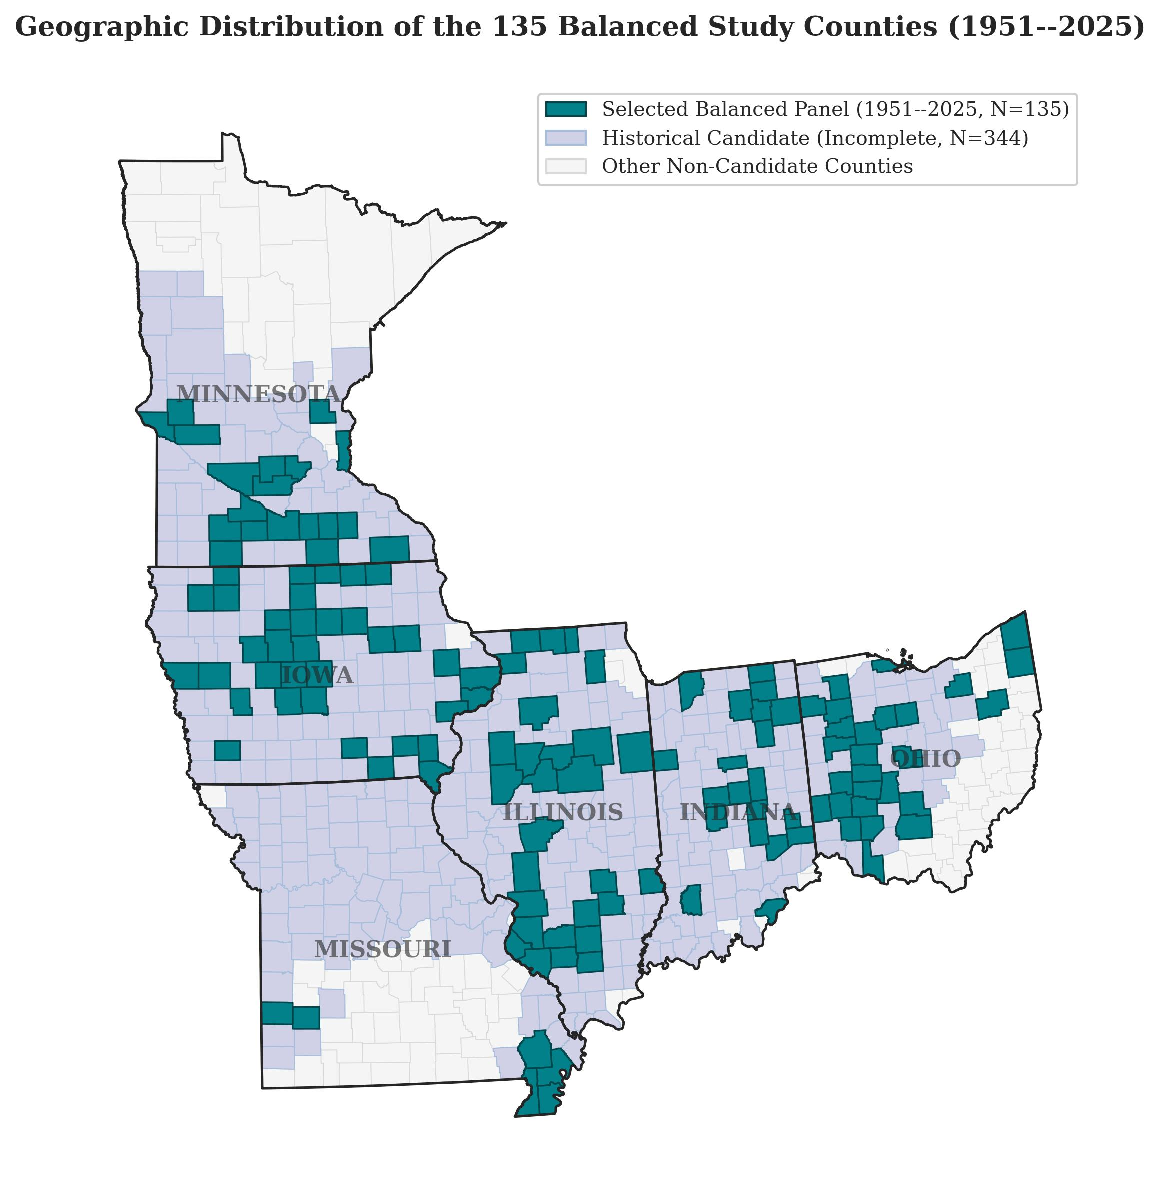
\includegraphics[width=0.92\textwidth]{figures/fig_study_area_map}
    \caption{Geographic distribution of the 135 balanced study counties across the six Midwestern states (1951--2025), illustrating balanced coverage across the primary agro-ecological subregions of the Corn and Soybean Belt.}
    \label{fig:study_area_map}
\end{figure}

\subsection{Soybean Phenology and Critical Agro-Climatic Sensitivity Windows}
\label{sec:data_phenology}

Soybean development spans approximately six months, initiating with sowing in late April or May and concluding with harvest in September or October \citep{FehrCaviness1977}. To capture how intra-seasonal meteorological anomalies propagate into realized yield shocks, the cultivation cycle is structured into four sequential operational and phenological phases:

\begin{enumerate}
    \item \textbf{Sowing, Germination, and Emergence (April--May):}
    Germination requires seedbed temperatures consistently above $10^\circ\text{C}$ along with adequate moisture for imbibition. While farmers aim to plant early (late April to early May) to maximize solar radiation capture during summer, prolonged exposure to saturated, cold soils ($<10^\circ\text{C}$) induces seed chilling injury, pathogen vulnerability, and soil compaction. Substantial planting delays into June compress the vegetative window and curtail overall yield potential.
    
    \item \textbf{Vegetative Growth and Canopy Closure (June, V1--Vn):}
    Following emergence, the crop undergoes rapid vegetative development, driven by thermal accumulation (Growing Degree Days, $GDD$), establishing trifoliate nodes and taproots into intermediate soil layers ($7$--$28\text{ cm}$). Moderate early moisture deficits encourage deeper root penetration, whereas severe drought or prolonged root-zone waterlogging stunting canopy closure permanently diminishes the photosynthetic capacity needed to support reproductive organs.
    
    \item \textbf{Mid-Summer Reproductive Peak and Pod-Filling (July--August, R1--R6):}
    The July--August window represents the critical biological bottleneck of the entire crop lifecycle \citep{Schlenker2009, Lobell2014}. In July (flowering and pod initiation, R1--R3), atmospheric maximum temperatures exceeding $30^\circ\text{C}$ and elevated vapor pressure deficits ($VPD > 1.5\text{ kPa}$) induce pollen sterility, reduce pollination efficiency, and trigger irreversible floral and pod abscission. In August (pod filling and seed enlargement, R4--R6), transpirational water demand peaks as assimilated carbon and nitrogen translocate into developing seeds. Severe heat or moisture deficits in August cause leaf senescence, pod abortion, and shriveled seeds, whereas abundant subsoil moisture and moderate temperatures maximize seed weight.
    
    \item \textbf{Maturation, Desiccation, and Harvest (September--October, R7--R8):}
    Upon reaching physiological maturity (R7), dry matter accumulation ceases, and seed moisture decreases from over $50\%$ toward harvest levels ($13\%$--$15\%$). Weather during this phase no longer influences biological yield potential, but dictates field workable days, combine efficiency, and mechanical harvest losses. Early hard autumn freezes ($T_{\text{min}} < 0^\circ\text{C}$) before R7 halt seed filling prematurely, while prolonged late-autumn rainfall induces lodging, pod shattering, and field access delays.
\end{enumerate}

\section{Exploratory Data Analysis of County Soybean Yields (1951--2025)}
\label{sec:data_eda}

\subsection{Secular Technological Trend, Productivity Tripling, and Anomaly Decomposition}
\label{sec:data_yield_decomposition}

To clarify the physical drivers of historical crop variation and formalize the empirical target, realized county soybean yield $y_{c,t}$ (bu/ac for county $c$ and year $t \in \{1951, \dots, 2025\}$) is decomposed into two orthogonal components:
\begin{equation}
    y_{c,t} = \tau_{c,t} + \epsilon_{c,t}
    \label{eq:yield_decomp_ch3}
\end{equation}
where $\tau_{c,t}$ represents the deterministic secular trend driven by cumulative technological, agronomic, and genetic innovations, and $\epsilon_{c,t}$ denotes the stochastic shock anomaly induced by intra-seasonal atmospheric forcing and environmental extremes.

\begin{figure}[htbp]
    \centering
    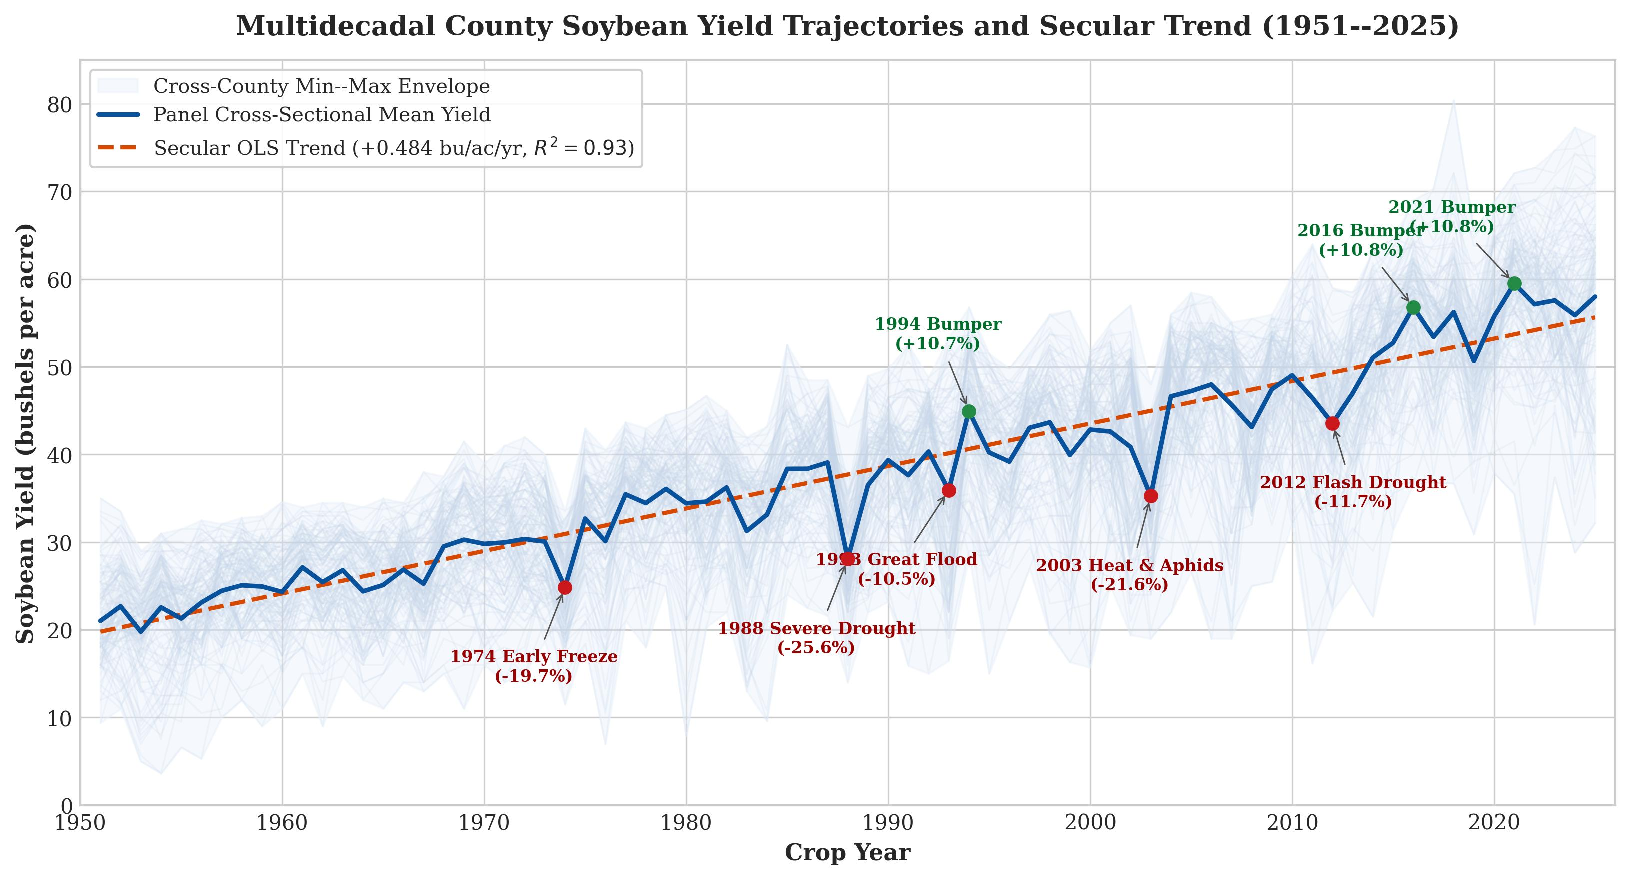
\includegraphics[width=0.96\textwidth]{figures/fig_yield_trajectory}
    \caption{Multidecadal county soybean yield trajectories and secular trend across 135 Midwestern counties (1951--2025). Light lines represent individual county histories; the solid blue line denotes the annual cross-sectional panel mean; the dashed line represents the secular OLS trend; and markers highlight major historical climatic shock anomalies.}
    \label{fig:yield_trajectory}
\end{figure}

The secular baseline $\tau_{c,t}$ captures steady technological progress, including breeding advancements (improved lodging resistance, optimized maturity groups), transgenic traits, farm mechanization, subsurface tile drainage, and precision crop inputs. Across the 75-year panel, regional soybean yields expanded from an unweighted mean of $22.77\text{ bu/ac}$ in the 1950s to $57.31\text{ bu/ac}$ in the 2020s, a net gain of $+151.7\%$ (Table~\ref{tab:decadal_yields}). A pooled linear secular trend accounts for over 81\% of total county-year yield variance ($R^2 = 0.8122$, $N = 10{,}125$). Aggregated to the annual regional mean ($N = 75$), an ordinary least squares regression yields an average rate of progress of $+0.484\text{ bu/ac/year}$ ($R^2 = 0.9323$):
\begin{equation}
    \hat{y}_t = 0.484 \cdot t - 925.46 \quad (t = 1951, \dots, 2025)
    \label{eq:panel_trend}
\end{equation}

% Table 3.2: Decadal Distributional Statistics of Soybean Yields (1951-2025)
\begin{table}[htbp]
\centering
\footnotesize
\setlength{\tabcolsep}{3.5pt}
\caption{Decadal distributional dynamics of Midwestern county-level soybean yields (1951--2025).}
\label{tab:decadal_yields}
\begin{tabular*}{\textwidth}{@{\extracolsep{\fill}}l c c c c c c c c}
\toprule
\textbf{Period} & \textbf{Obs.} & \textbf{Mean} & \textbf{Median} & \textbf{Std. Dev.} & \textbf{Min} & \textbf{Max} & \textbf{IQR} & \textbf{CV} \\
 & ($N$) & (bu/ac) & (bu/ac) & (bu/ac) & (bu/ac) & (bu/ac) & (bu/ac) & (\%) \\
\midrule
1950s (1951--1959) & 1,215 & 22.77 & 23.10 & 5.01 & 3.6 & 35.0 & 6.55 & 22.0\% \\
1960s (1960--1969) & 1,350 & 26.51 & 26.60 & 5.07 & 9.0 & 41.5 & 6.98 & 19.1\% \\
1970s (1970--1979) & 1,350 & 31.38 & 32.00 & 6.04 & 7.0 & 44.5 & 8.90 & 19.2\% \\
1980s (1980--1989) & 1,350 & 35.01 & 35.75 & 6.63 & 7.9 & 52.5 & 8.58 & 19.0\% \\
1990s (1990--1999) & 1,350 & 40.43 & 41.50 & 7.08 & 15.0 & 56.8 & 9.27 & 17.5\% \\
2000s (2000--2009) & 1,350 & 43.97 & 45.00 & 7.78 & 15.7 & 58.5 & 11.20 & 17.7\% \\
2010s (2010--2019) & 1,350 & 50.70 & 51.40 & 7.80 & 16.2 & 80.4 & 10.00 & 15.4\% \\
2020s (2020--2025) & 810 & 57.31 & 57.95 & 7.57 & 20.6 & 77.3 & 9.65 & 13.2\% \\
\midrule
\textbf{Full Panel (1951--2025)} & \textbf{10,125} & \textbf{37.72} & \textbf{36.70} & \textbf{12.40} & \textbf{3.6} & \textbf{80.4} & \textbf{19.00} & \textbf{32.9\%} \\
\bottomrule
\end{tabular*}
\vspace{1ex}
\raggedright
\footnotesize{\textit{Notes:} Yields are measured in bushels per acre (bu/ac). Obs. denotes total county-year observations in each period (135 counties $\times$ years). IQR is the interquartile range ($Q_3 - Q_1$). CV is the coefficient of variation ($100 \times \sigma / \mu$). Note the systematic decrease in CV from 22.0\% in the 1950s to 13.2\% in the 2020s despite an increase in absolute standard deviation.}
\end{table}


From a supply-chain and modeling perspective, separating $\tau_{c,t}$ from $\epsilon_{c,t}$ is crucial. While the secular trajectory is readily anticipated by market actors and capitalized into logistics capacity, systemic commodity volatility and supply shortfalls are driven by the weather-induced anomaly $\epsilon_{c,t}$. Furthermore, because baseline yields have nearly tripled, a given percentage drought shock corresponds to a substantially larger physical volume loss today than in the 1950s.

A deterministic linear specification provides a parsimonious, robust baseline that eliminates Runge-type endpoint oscillations and avoids overfitting the multi-year climate cycles that flexible non-parametric filters inadvertently absorb \citep{Schlenker2009, Lobell2014}. The formal mathematical estimation of candidate detrending models, penalization schemes, and strict train-only expanding-window implementations is formalized in the predictive methodology of Chapter~4.

\subsection{Spatial Heterogeneity and Regional Productivity Divergence}

While the secular trend is positive across the entire Midwest, regional productivity exhibits pronounced spatial heterogeneity across states and agro-climatic zones. Figure~\ref{fig:state_yield_distributions} contrasts the cross-sectional yield distributions and decadal trajectories across the six states.

\begin{figure}[htbp]
    \centering
    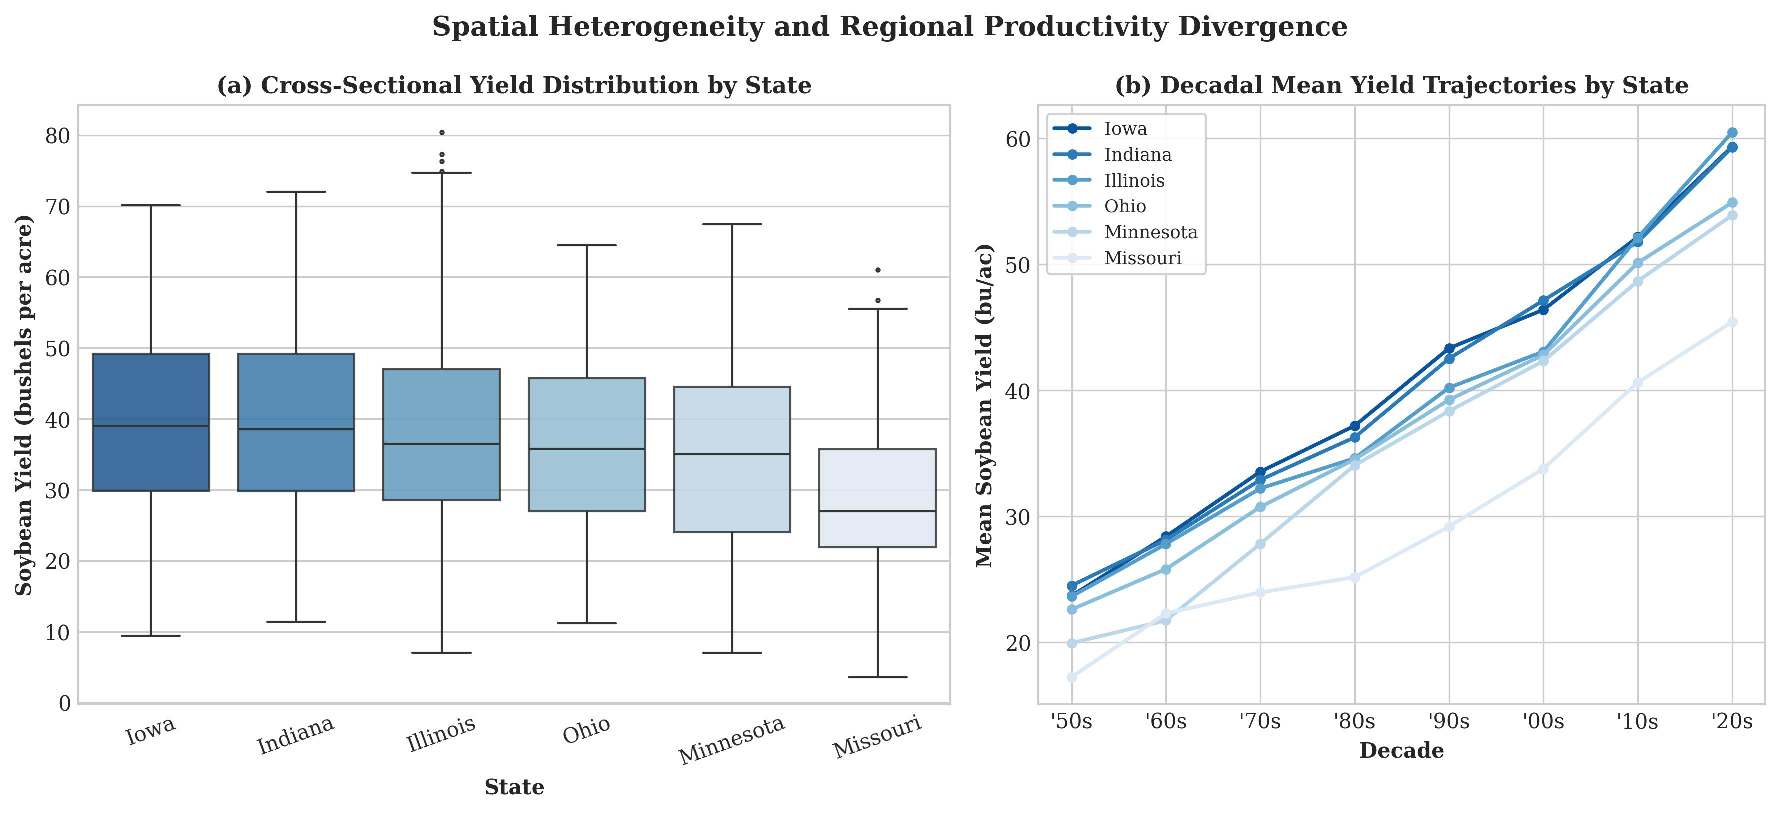
\includegraphics[width=0.96\textwidth]{figures/fig_state_yield_distributions}
    \caption{Spatial heterogeneity of county soybean yields: (a) cross-sectional yield distributions by state ordered by median yield; (b) decadal mean yield trajectories across the six Midwestern states from the 1950s to the 2020s.}
    \label{fig:state_yield_distributions}
\end{figure}

Iowa (mean yield $39.73\text{ bu/ac}$; secular trend $+0.495\text{ bu/ac/year}$) and Illinois (mean $38.35\text{ bu/ac}$; trend $+0.491\text{ bu/ac/year}$) form the high-yielding core of the Corn Belt, underpinned by deep prairie soils with superior moisture-retention capacities. Indiana ($39.52\text{ bu/ac}$) and western Ohio ($36.88\text{ bu/ac}$) exhibit comparable productivity with lower cross-county dispersion. 

In contrast, Minnesota presents a lower historical mean ($35.10\text{ bu/ac}$) but the fastest linear growth rate in the panel ($+0.509\text{ bu/ac/year}$). This rapid acceleration reflects the northward migration of soybean acreage during the late 20th century, made possible by the commercial development of cold-tolerant, short-season cultivars (maturity groups 0 and 00) and warmer spring temperatures. At the southern fringe, Missouri displays both the lowest historical yield level ($29.04\text{ bu/ac}$) and the lowest trend slope ($+0.386\text{ bu/ac/year}$), driven by shallower topsoils (claypan subsoils) and elevated susceptibility to summer heatwaves and dry spells.

\subsection{Dispersion Dynamics: Absolute Variance vs. Relative Volatility}

A fundamental question in agricultural risk analysis is whether technological modernization has altered crop vulnerability to environmental shocks. Figure~\ref{fig:dispersion_dynamics} resolves this by examining absolute cross-county standard deviation ($\sigma_t$) alongside relative volatility, measured by the coefficient of variation ($CV_t = 100 \times \sigma_t / \mu_t$).

\begin{figure}[htbp]
    \centering
    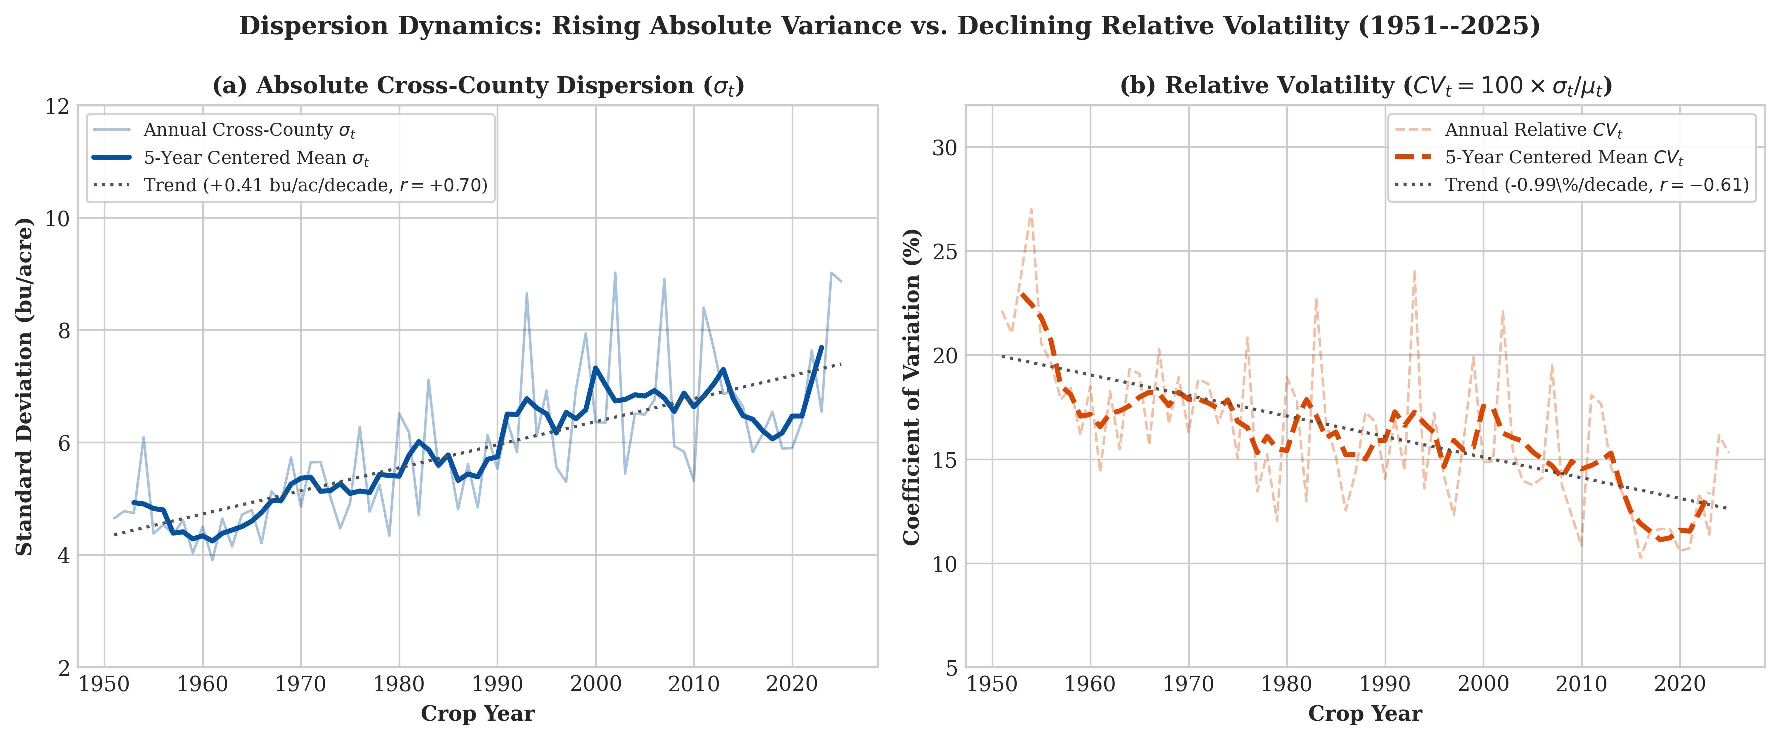
\includegraphics[width=0.90\textwidth]{figures/fig_dispersion_dynamics}
    \caption{Dispersion dynamics across the 135 Midwestern study counties (1951--2025). The blue curves illustrate rising absolute cross-county standard deviation ($\sigma_t$, left axis), while the dashed orange curves depict steadily declining relative coefficient of variation ($CV_t$, right axis). Solid thick lines denote 5-year centered rolling averages.}
    \label{fig:dispersion_dynamics}
\end{figure}

The empirical evidence reveals a clear dichotomy: while absolute standard deviation has expanded from $5.01\text{ bu/ac}$ in the 1950s to $7.57\text{ bu/ac}$ in the 2020s ($r = +0.705$), the coefficient of variation has declined systematically from $22.0\%$ to $13.2\%$ ($r = -0.610$, Table~\ref{tab:decadal_yields}). Modern cultivars, seed treatments, and drainage have dampened \textit{relative} vulnerability to localized micro-stresses. However, because baseline yield levels have nearly tripled, the \textit{absolute} bushel shortfall generated during severe regional droughts is substantially larger today, heightening volume exposure for commercial supply-chain logistics.

\subsection{Macro-Climatic Historical Yield Shocks and Biological Asymmetry}
\label{sec:data_yield_shocks}

The 75-year panel captures prominent macro-climatic shock campaigns that serve as out-of-sample benchmark years. Using an asymmetric anomaly threshold of $|\epsilon_t / \hat{y}_t| \ge 10\%$ relative to the secular trend, Table~\ref{tab:yield_shocks} classifies historical extreme campaigns into adverse shortfalls and favorable bumper regimes alongside their dominant hazard archetypes.

% Table 3.3: Historical Macro-Climatic Yield Shocks in the Midwestern Panel (1951-2025)
\begin{table}[htbp]
\centering
\small
\caption{Historical macro-climatic shock years and associated meteorological drivers (1951--2025).}
\label{tab:yield_shocks}
\begin{tabularx}{\textwidth}{c c c c c X}
\toprule
\textbf{Year} & \textbf{Observed} & \textbf{Trend} & \textbf{Anomaly} & \textbf{Rel. Anomaly} & \textbf{Primary Meteorological / Ecological Driver} \\
 & (bu/ac) & (bu/ac) & (bu/ac) & (\%) & \\
\midrule
\multicolumn{6}{l}{\textit{\textbf{Panel A: Major Adverse Macro-Climatic Yield Shocks (Negative Anomalies)}}} \\[0.5ex]
1988 & 28.08 & 37.72 & -9.64 & -25.6\% & Historic severe summer drought and persistent heatwave across the Corn Belt. \\
2003 & 35.26 & 44.98 & -9.72 & -21.6\% & Late-summer heat and moisture stress compounded by widespread soybean aphid outbreak. \\
1974 & 24.84 & 30.93 & -6.09 & -19.7\% & Excessively wet spring delaying planting, followed by mid-summer drought and early September frost. \\
2012 & 43.55 & 49.34 & -5.80 & -11.7\% & Extensive summer flash drought and record July heat across the central United States. \\
1983 & 31.27 & 35.29 & -4.02 & -11.4\% & Prolonged July-August heatwave and severe drought across the Corn and Soybean Belt. \\
1993 & 35.92 & 40.14 & -4.22 & -10.5\% & Great Upper Mississippi River flood; prolonged waterlogging, root asphyxia, and disease. \\
\midrule
\multicolumn{6}{l}{\textit{\textbf{Panel B: Prominent Favorable Bumper Harvests (Positive Anomalies)}}} \\[0.5ex]
1952 & 22.69 & 20.27 & +2.41 & +11.9\% & Exceptionally favorable vegetative and pod-filling moisture across the central belt. \\
2021 & 59.50 & 53.70 & +5.79 & +10.8\% & Optimal reproductive rainfall and moderate temperatures throughout August. \\
2016 & 56.81 & 51.28 & +5.53 & +10.8\% & Broadly distributed summer rains and minimal extreme heat stress across the Midwest. \\
1994 & 44.95 & 40.62 & +4.33 & +10.7\% & Record-setting benign growing conditions with timely August rains and cool nights. \\
\bottomrule
\end{tabularx}
\vspace{1ex}
\raggedright
\footnotesize{\textit{Notes:} Observed represents the unweighted cross-sectional mean yield of all 135 panel counties. Trend is estimated via linear OLS over 1951--2025 ($\hat{y}_t = 0.484t - 925.46$). Anomaly is $y_t - \hat{y}_t$, and Rel. Anomaly is $(y_t - \hat{y}_t)/\hat{y}_t \times 100$. Note that 1988 represents the deepest shortfall in the 75-year record ($-25.6\%$), while 1993 highlights non-drought atmospheric hazards (excess precipitation and soil saturation).}
\end{table}


The empirical distribution of extreme yield anomalies exhibits pronounced \textbf{biological and statistical asymmetry}. Favorable bumper harvests cluster tightly within a narrow upper bound ($+10.1\%$ to $+11.9\%$; e.g., 1952, 1961, 1994, 2016, 2021). Under optimal weather, dry matter accumulation is bounded by an asymptotic physiological ceiling governed by RuBisCO carboxylation kinetics, canopy radiation interception, and genetic sink strength. 

Conversely, adverse abiotic stressors possess no physiological floor short of total crop loss, generating an elongated lower tail down to $-19.7\%$ (1974), $-21.6\%$ (2003), and $-25.6\%$ (1988), producing significant negative skewness ($-1.12$, Jarque-Bera test $p < 0.001$). As cataloged in Table~\ref{tab:yield_shocks}, these severe downside shocks reflect distinct compound hazards:
\begin{itemize}
    \item \textit{Compound Thermal-Drought Stress (1953, 1983, 1988, 2012):} High temperatures ($T_{\text{max}} > 30^\circ\text{C}$ and $>35^\circ\text{C}$) coupled with elevated vapor pressure deficits ($VPD > 1.8\text{ kPa}$) induce pollen sterility, floral abscission, and transpirational collapse \citep{Schlenker2009, Lobell2014}.
    \item \textit{Pluvial Inundation and Soil Anoxia (1993):} Persistent waterlogging causes root-zone oxygen deprivation, impairs symbiotic nitrogen fixation, and fosters fungal diseases, cutting yields by $-10.5\%$ in the absence of drought.
    \item \textit{Planting Delays and Early Frost (1974):} Wet spring conditions delay planting into June, pushing pod fill late into summer and exposing immature crops to early autumn freezes ($-19.7\%$).
    \item \textit{Compound Biotic-Abiotic Stress (2003):} Late-summer moisture deficits interact synergistically with aphid outbreaks, exacerbating losses ($-21.6\%$).
\end{itemize}

Crucially, because synoptic weather patterns span hundreds of kilometers, meteorological anomalies affect contiguous counties simultaneously. Within our panel, cross-county detrended yield correlations average above $0.75$, highlighting strong spatial autocorrelation and necessitating strict year-based temporal cross-validation to prevent spatial leakage \citep{Sweetetal2023}.

% ==============================================================================
% PART 2: ATMOSPHERIC REANALYSIS AND AGRO-CLIMATIC SENSITIVITY
% ==============================================================================

\section{Atmospheric Reanalysis: ECMWF ERA5-Land}
\label{sec:data_era5}

\subsection{Methodological Rationale for a Weather-Only Scope}
\label{sec:data_weather_only_rationale}

The empirical predictive framework restricts dynamic predictive inputs strictly to gridded surface weather from ECMWF ERA5-Land \citep{MunozSabater2021}, which provides continuous, physically consistent hourly meteorological fields at $0.1^\circ \times 0.1^\circ$ resolution ($\approx 9\text{ km}$ across the Midwest), free from station-discontinuation artifacts and spatial interpolation gaps.

As theoretically grounded in Chapter~\ref{chap:literature_review}, this weather-only constraint is dictated by operational real-time requirements and multidecadal data integrity:
\begin{enumerate}
    \item \textbf{Operational Feasibility and Lag Elimination:} County-level management records (planting dates, fertilizer rates, cultivar adoptions) are compiled ex-post and released months after harvest, making them inadmissible for real-time forecasting. Furthermore, consistent 75-year historical records do not exist.
    \item \textbf{Historical Depth and Satellite Latency:} Remote sensing greenness proxies (MODIS/Sentinel NDVI, EVI, SIF) are available only post-2000, preventing multidecadal sampling of climatic extremes. Moreover, optical indices exhibit severe physiological latency, offering no predictive utility during pre-sowing and early vegetative windows ($H \ge 4$).
    \item \textbf{Zero Temporal Variance of Static Soil Grids:} While soil properties (SSURGO available water capacity, texture) help establish spatial baseline productivity, their values are temporally invariant ($\text{Var}(X_{it}) = 0$) and cannot explain interannual yield shocks.
    \item \textbf{Unconfounded Physical Benchmark:} Coupling yield models with dynamical seasonal climate forecasts (e.g., SEAS5) conflates crop response functions with climate model forecast drift and systematic biases. Restricting inputs to realized surface reanalysis establishes the empirical upper bound of predictability attributable strictly to observed atmospheric forcing up to each forecast cutoff.
\end{enumerate}

\subsection{Spatial Aggregation: Exact Planar Polygon Intersection}

To map gridded reanalysis fields into irregularly shaped administrative county polygons, an exact planar polygon-intersection geometry was computed (\texttt{spatial\_weights.csv}). Across the 135 counties and the ERA5-Land $0.1^\circ$ grid, 3,344 unique intersection polygons are identified with normalized area weights:
\begin{equation}
    w_{c,g} = \frac{\text{Area}(c \cap g)}{\text{Area}(c)}, \quad \sum_{g \in \mathcal{G}_c} w_{c,g} = 1
    \label{eq:spatial_weight}
\end{equation}
where $\text{Area}(c \cap g)$ is the planar intersection area between county polygon $c$ and grid cell $g$, and $\mathcal{G}_c$ denotes the set of intersecting grid cells.

This area-weighted polygon integration represents a significant methodological advance over naive centroid sampling. Centroid extraction assumes that a single point can represent an entire county, which introduces severe spatial sampling errors in large Midwestern counties characterized by localized convective precipitation gradients and heterogeneous topography. Exact area weighting accurately integrates the total atmospheric mass, radiation, and precipitation volume falling within county boundaries.

\subsection{Temporal Aggregation and Crop Campaign Structure}

Hourly ERA5-Land reanalysis fields are spatially aggregated via Equation~\eqref{eq:spatial_weight} and summarized into daily indicators:
\begin{itemize}
    \item \textbf{Thermodynamic States:} Daily mean, maximum, and minimum 2m air temperature ($T_{\text{mean}}, T_{\text{max}}, T_{\text{min}}$), daily mean 2m dewpoint ($T_{\text{dew}}$), and daily mean/maximum skin temperature ($T_{\text{skt}}$) in $^\circ$C.
    \item \textbf{Cumulative Fluxes:} Daily cumulative precipitation ($P$, mm/day), surface solar radiation downwards ($SSRD$, $\text{MJ}/\text{m}^2/\text{day}$), and surface thermal radiation downwards ($STRD$, $\text{MJ}/\text{m}^2/\text{day}$).
    \item \textbf{Boundary Layer and Wind Dynamics:} Daily mean surface pressure ($SP$, kPa), 10m horizontal wind components ($u_{10}, v_{10}$, m/s), and scalar wind speed ($WS_{10}$, m/s).
    \item \textbf{Pedological State Variables:} Daily mean soil temperature across four discrete depth horizons ($STL_1$--$STL_4$: $0$--$7$, $7$--$28$, $28$--$100$, and $100$--$289\text{ cm}$, $^\circ$C), and volumetric soil moisture across the same four horizons ($SM_1$--$SM_4$, $\text{m}^3/\text{m}^3$).
\end{itemize}

For each crop year $Y$, daily weather processing is structured over a 13-month campaign spanning from October 1 of year $Y-1$ to October 31 of year $Y$ (397 consecutive days). This multi-month temporal structure aligns with the 12 progressive monthly forecast horizons ($H=12, \dots, 1$) evaluated on the last day of each month, capturing antecedent overwinter soil moisture recharge and growing-season atmospheric forcing without temporal data leakage.

\subsection{Derived Agrometeorological Variables and Bioclimatic Indicators}
\label{sec:data_derived_weather}

Because crop physiological response functions operate non-linearly on compound atmospheric-hydrological demands rather than isolated averages \citep{Schlenker2009, Hoffman2020}, raw ERA5-Land fields are processed into primary and derived daily agrometeorological indicators (Table~\ref{tab:weather_variables}).

\begin{table}[htbp]
\centering
\footnotesize
\setlength{\tabcolsep}{4pt}
\renewcommand{\arraystretch}{1.15}
\caption{ERA5-Land surface meteorological variables and derived daily agrometeorological indicators.}
\label{tab:weather_variables}
\begin{tabularx}{\textwidth}{p{2.3cm} p{2.8cm} p{1.3cm} X}
\toprule
\textbf{Category} & \textbf{Symbol} & \textbf{Unit} & \textbf{Physical Description and Agronomic Rationale} \\
\midrule
\multicolumn{4}{l}{\textit{Panel A: Primary Atmospheric and Land-Surface Reanalysis Fields (ECMWF ERA5-Land)}} \\
Thermal Dynamics & $T_{\text{mean}}, T_{\text{max}}, T_{\text{min}}$ & $^\circ$C & Daily mean, maximum, and minimum 2\,m air temperature; thermal accumulation and heat stress. \\
& $T_{\text{dew}}$ & $^\circ$C & Daily mean 2\,m dewpoint temperature; near-surface moisture baseline. \\
Hydrological Fluxes & $P$ & mm/d & Total daily precipitation; surface water supply, recharge, and waterlogging. \\
& $PE$ & mm/d & Potential evaporation; atmospheric evaporative capacity from the surface. \\
Radiative Forcing & $SSRD$ & $\text{MJ}/\text{m}^2/\text{d}$ & Surface downward solar radiation; photosynthetically active radiation driving biomass assimilation. \\
Pedological Moisture & $SM_1, SM_2, SM_3$ & $\text{m}^3/\text{m}^3$ & Volumetric soil water across depths: $0$--$7\text{ cm}$ (seedbed), $7$--$28\text{ cm}$ (upper root zone), and $28$--$100\text{ cm}$ (deep root reservoir). \\
\midrule
\multicolumn{4}{l}{\textit{Panel B: Derived Agrometeorological and Bioclimatic Indicators}} \\
Evaporative Demand & $VPD$ & kPa & Vapor pressure deficit $e_s(T_{\text{mean}}) - e_a(T_{\text{dew}})$; atmospheric drying power driving stomatal closure. \\
Crop Water Demand & $ET_0$ & mm/d & FAO-56 Penman-Monteith reference evapotranspiration \citep{Allen1998}. \\
Climatic Balance & $P - ET_0$ & mm/d & Climatic water balance; net daily atmospheric moisture deficit or surplus. \\
Thermal Pacing & $GDD$ & $^\circ$C$\cdot$d & Growing Degree Days ($10$--$30^\circ$C); vegetative and reproductive phenological progression pacing. \\
Extreme Heat Stress & $HD_{30}, HD_{35}$ & binary & Daily heat day exceedances $\mathbb{I}(T_{\text{max}} \ge 30^\circ\text{C})$ and $\ge 35^\circ\text{C}$ \citep{Schlenker2009}. \\
Root-Zone Reservoir & $SM_{\text{root}}$ & $\text{m}^3/\text{m}^3$ & Depth-weighted soil water column ($0$--$100\text{ cm}$, Eq.~\eqref{eq:sm_root}); multi-month hydrological buffer. \\
\bottomrule
\end{tabularx}
\end{table}


\paragraph{Vapor Pressure Deficit ($VPD$).} Atmospheric evaporative demand is parameterized via Vapor Pressure Deficit, which quantifies the drying power of the air. Saturation vapor pressure $e_s(T_{\text{mean}})$ and actual vapor pressure $e_a(T_{\text{dew}})$ (in kPa) are computed via Tetens formulations:
\begin{align}
    e_s(T_{\text{mean}}) &= 0.61078 \exp\left( \frac{17.27 \, T_{\text{mean}}}{T_{\text{mean}} + 237.3} \right), \quad
    e_a(T_{\text{dew}}) = 0.61078 \exp\left( \frac{17.27 \, T_{\text{dew}}}{T_{\text{dew}} + 237.3} \right) \label{eq:tetens} \\
    VPD &= \max\left(0, \, e_s(T_{\text{mean}}) - e_a(T_{\text{dew}})\right) \label{eq:vpd}
\end{align}
Elevated $VPD$ ($>1.5\text{ kPa}$) triggers stomatal closure to prevent xylem cavitation, suppressing transpirational cooling and carbon assimilation during reproductive stages \citep{Grossiord2020, Lobell2014}.

\paragraph{Reference Evapotranspiration ($ET_0$) and Climatic Water Balance ($P - ET_0$).} Potential atmospheric water demand is modeled via the standardized FAO-56 Penman-Monteith equation for a short grass reference canopy \citep{Allen1998}:
\begin{equation}
    ET_0 = \frac{0.408 \, \Delta \, (R_n - G) + \gamma \, \frac{900}{T_{\text{mean}} + 273} \, u_2 \, (e_s - e_a)}{\Delta + \gamma \, (1 + 0.34 \, u_2)}
    \label{eq:penman_monteith}
\end{equation}
where $R_n$ is net surface radiation ($\text{MJ}/\text{m}^2/\text{day}$), $G \approx 0$ is daily soil heat flux density, $u_2$ is 2m wind speed ($\text{m/s}$), $\Delta$ is the saturation vapor pressure slope, and $\gamma$ is the psychrometric constant. Daily climatic water balance tracks atmospheric moisture deficits or recharge surpluses:
\begin{equation}
    P_{\text{net}} = P - ET_0
    \label{eq:climatic_balance}
\end{equation}

\paragraph{Thermal Pacing and Extreme Heat Days ($GDD, HD_{30}, HD_{35}$).} Phenological progression is tracked through Growing Degree Days ($GDD$, base $10^\circ\text{C}$, cap $30^\circ\text{C}$):
\begin{equation}
    GDD = \max\left(0, \, \frac{\min(T_{\text{max}}, 30) + \max(T_{\text{min}}, 10)}{2} - 10\right)
    \label{eq:gdd}
\end{equation}
To capture non-linear thermal damage thresholds \citep{Schlenker2009}, extreme heat exposure is quantified via daily exceedances:
\begin{equation}
    HD_{30} = \max(0, \, T_{\text{max}} - 30), \quad HD_{35} = \max(0, \, T_{\text{max}} - 35)
    \label{eq:heat_days}
\end{equation}
alongside binary daily occurrences $\mathbb{I}(T_{\text{max}} \ge 30^\circ\text{C})$ and $\mathbb{I}(T_{\text{max}} \ge 35^\circ\text{C})$.

\paragraph{Integrated Root-Zone Soil Moisture ($SM_{\text{root}}$).} Volumetric soil moisture across discrete depth horizons is aggregated into an integrated column accessible to mature soybean taproots ($0$--$100\text{ cm}$):
\begin{equation}
    SM_{\text{root}} = 0.07 \, SM_1 + 0.21 \, SM_2 + 0.72 \, SM_3
    \label{eq:sm_root}
\end{equation}
weighting by layer thickness ($7\text{ cm}$, $21\text{ cm}$, $72\text{ cm}$). This metric buffers transient surface dry spells and tracks subsoil moisture memory sustaining transpirational uptake during summer rainfall deficits \citep{Vijverberg2023}.

\section{Exploratory Agro-Climatic Analysis and Yield Sensitivity}
\label{sec:data_climate_eda}

\subsection{Baseline Climatology and Intra-Annual Seasonality}
\label{sec:data_seasonality}

Before examining multi-decadal historical shocks, it is essential to establish the intra-annual baseline climatology that governs crop development across the Midwestern Corn Belt. Utilizing the daily spatially weighted ERA5-Land reanalysis across the 135 study counties over the 1950--present record, Figure~\ref{fig:weather_seasonality} characterizes the seasonal progression of thermal regimes, cumulative water balances, and edaphic moisture depletion across the primary soybean growing cycle (April 1 to October 31).

\begin{figure}[htbp]
    \centering
    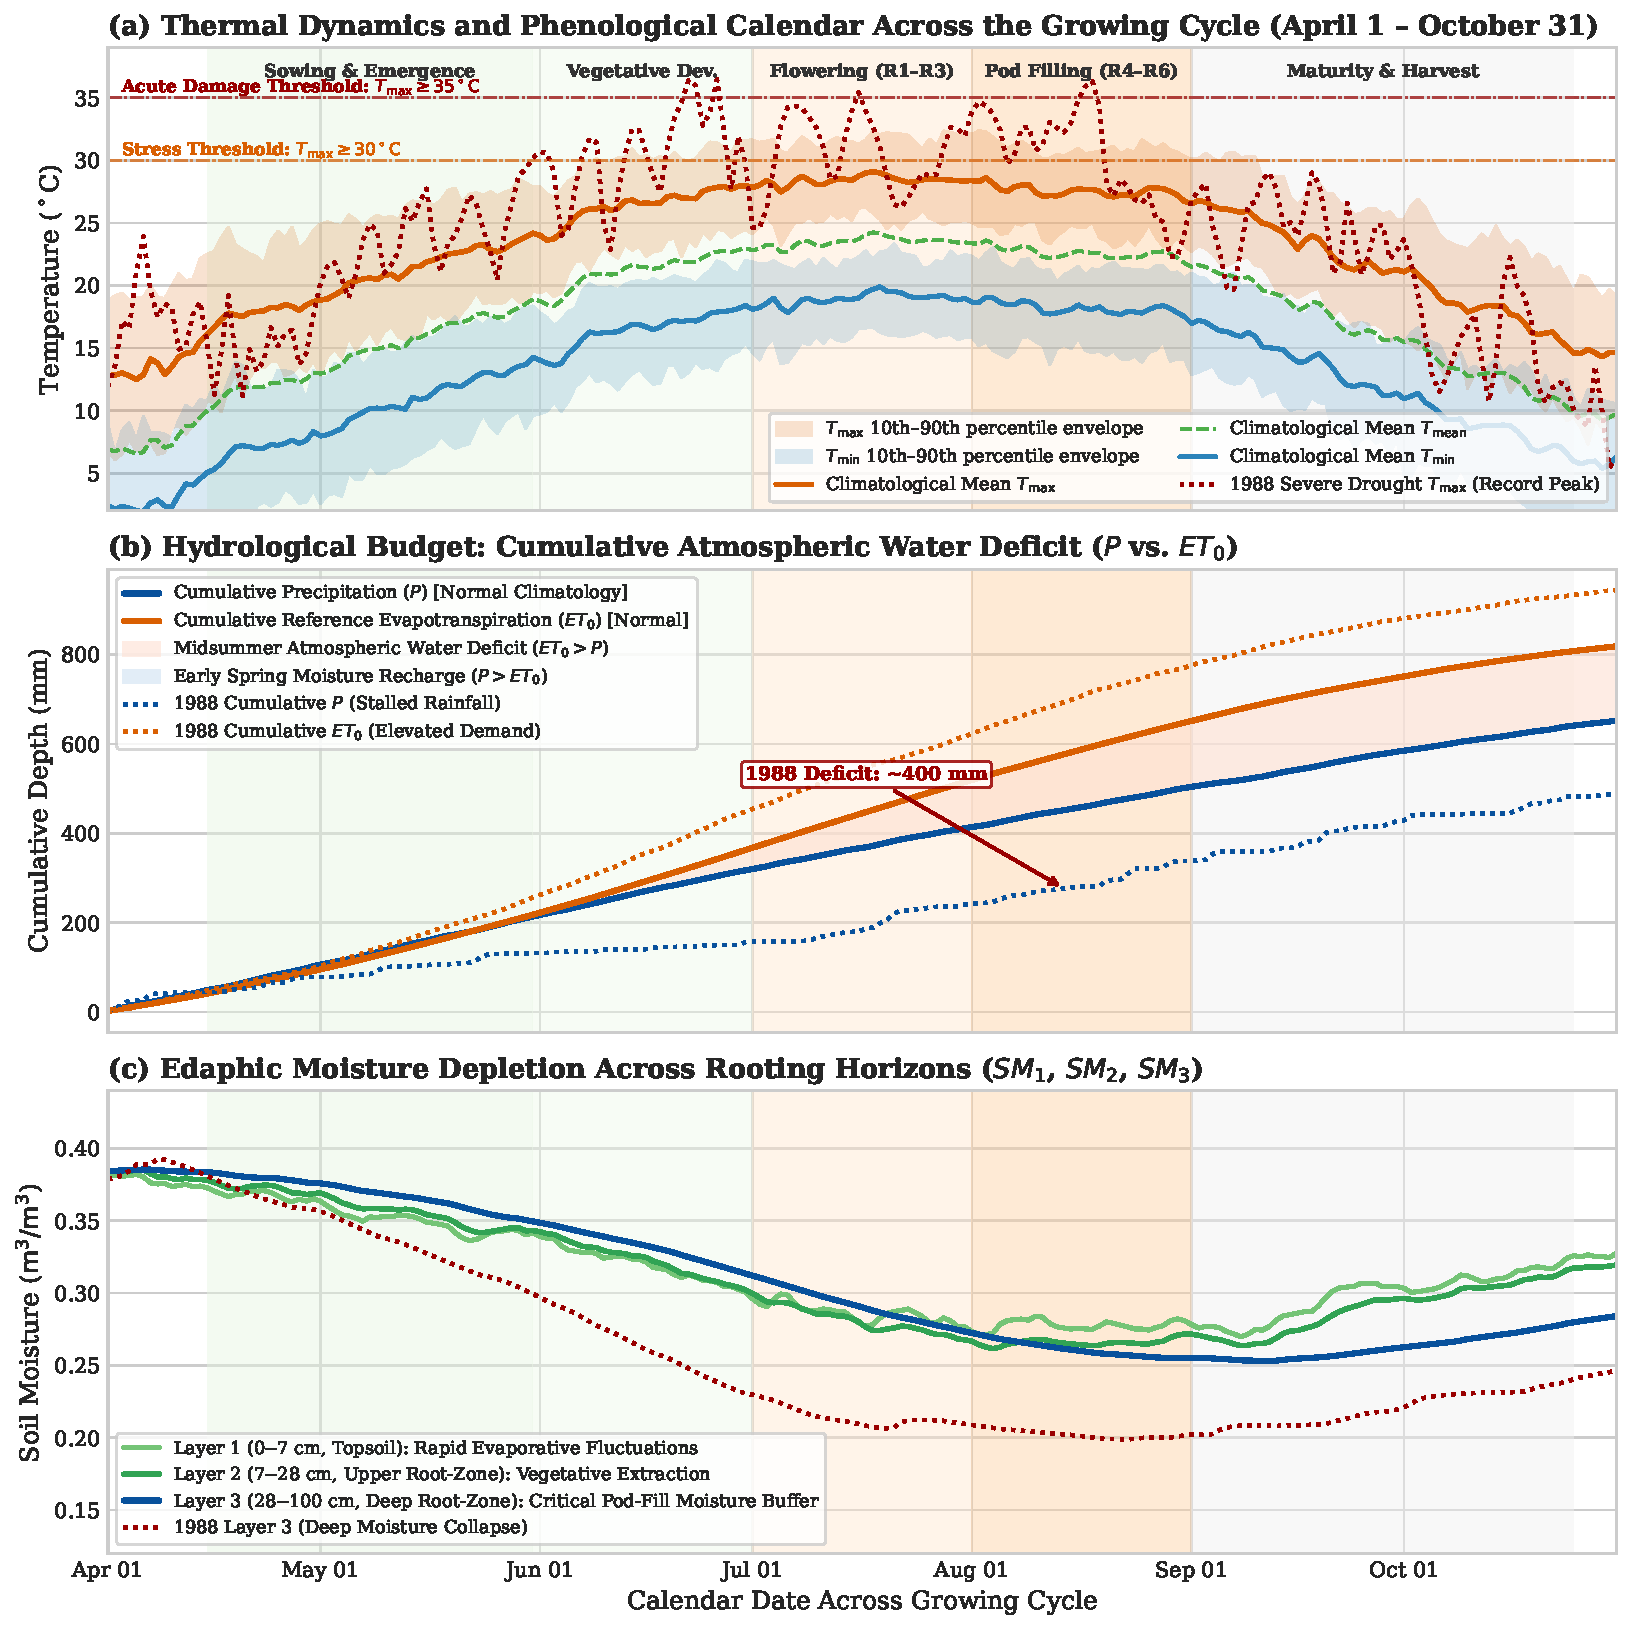
\includegraphics[width=0.96\textwidth]{figures/fig_weather_seasonality}
    \caption{Midwestern agro-climatic seasonality and intra-annual phenological dynamics across the 135 study counties (April 1 to October 31). Panel (a) illustrates daily thermal dynamics ($T_{\text{max}}, T_{\text{mean}}, T_{\text{min}}$) alongside 10th--90th percentile envelopes and cardinal damage thresholds ($30^\circ\text{C}$ and $35^\circ\text{C}$), contrasted against the record 1988 severe drought. Vertical shaded bands demarcate the five standardized phenological development stages. Panel (b) depicts the cumulative hydrological budget, highlighting the emergence of the midsummer atmospheric water deficit ($ET_0 > P$) in July and August. Panel (c) tracks volumetric soil moisture depletion across discrete rooting horizons ($SM_1$, $SM_2$, $SM_3$), demonstrating the essential buffering capacity of the deep root zone ($28$--$100\text{ cm}$).}
    \label{fig:weather_seasonality}
\end{figure}

The empirical intra-annual climatology synthesizes three foundational agronomic mechanisms across the developmental windows established in Section~\ref{sec:data_phenology}:

First, daily thermal progression (Figure~\ref{fig:weather_seasonality}a) aligns with the biological cardinal boundaries of the soybean plant. During the pre-sowing and emergence window (April 15--May 31), mean ambient temperatures rise from $8^\circ\text{C}$ to $18^\circ\text{C}$, safely exceeding the biological base germination threshold ($T_{\text{base}} = 10^\circ\text{C}$). Across the 75-year climatological record (1951--2025), summer maximum temperatures ($T_{\text{max}}$) peak in mid-July at $28.5^\circ\text{C}$ with an interdecile envelope bounded between $24^\circ\text{C}$ and $32^\circ\text{C}$. In contrast, during historical drought cohorts—exemplified by 1953, 1983, 1988, and 2012—daily maxima consistently pierced above the $30^\circ\text{C}$ floral abortion threshold and repeatedly exceeded the $35^\circ\text{C}$ acute damage ceiling throughout flowering (R1--R3) and early pod set. Conversely, during prominent bumper harvest cohorts such as 1952, 1961, 1994, 2016, and 2021, summer maxima remained consistently mild (hovering between $25^\circ\text{C}$ and $28^\circ\text{C}$), completely preventing canopy heat stress.

Second, the cumulative hydrological budget (Figure~\ref{fig:weather_seasonality}b) reveals the emergence of a structural midsummer atmospheric water deficit. In early spring (April and May), cumulative precipitation ($P \approx 200\text{ mm}$) exceeds reference crop evapotranspiration ($ET_0 \approx 180\text{ mm}$), ensuring robust topsoil recharge. However, starting in mid-June and accelerating throughout July and August, rising net radiation and vapor pressure deficits drive cumulative $ET_0$ to surge past cumulative rainfall. Under normal climatological conditions, a net seasonal atmospheric moisture deficit of $\approx 180\text{ mm}$ opens between $ET_0$ ($820\text{ mm}$) and $P$ ($640\text{ mm}$). During acute drought events like 1988 and 2012, rainfall stalled at barely $400$--$450\text{ mm}$ while evaporative demand exceeded $920\text{ mm}$, opening an unprecedented atmospheric moisture deficit of over $400\text{ mm}$. In contrast, bumper campaigns benefit from timely, well-distributed convective rainfall events that maintain cumulative deficits near a moderate equilibrium.

Third, the edaphic moisture profile (Figure~\ref{fig:weather_seasonality}c) demonstrates the critical buffering role of deep soil horizons. Volumetric moisture in the thin topsoil layer ($SM_1$, $0$--$7\text{ cm}$) exhibits erratic, high-frequency fluctuations driven by individual convective precipitation pulses and rapid surface evaporation. The intermediate layer ($SM_2$, $7$--$28\text{ cm}$) undergoes rapid extraction during vegetative expansion in June. Consequently, during the critical reproductive pod-filling phase in August (R4--R6), the crop becomes overwhelmingly reliant on the deep root-zone moisture reservoir ($SM_3$, $28$--$100\text{ cm}$). In normal seasons and bumper years, $SM_3$ declines smoothly from $0.38$ to $0.26\text{ m}^3/\text{m}^3$, providing a stable moisture buffer. In severe drought campaigns (such as 1988 and 1983), transpirational demand completely depleted $SM_3$ down to $0.18\text{ m}^3/\text{m}^3$, driving the soil column near the permanent wilting point and inducing widespread canopy desiccation.

\subsection{Historical Agro-Climatic Stress and the Yield Shock Nexus (1950--Present)}
\label{sec:data_climatology}

While intra-annual seasonality describes the average seasonal trajectory, interannual yield volatility is governed by the occurrence of acute atmospheric shocks. Figure~\ref{fig:weather_climatology} synchronizes the 75-year panel yield anomalies with the multi-decadal time series of atmospheric heat stress and evaporative demand across the 135 study counties.

\begin{figure}[htbp]
    \centering
    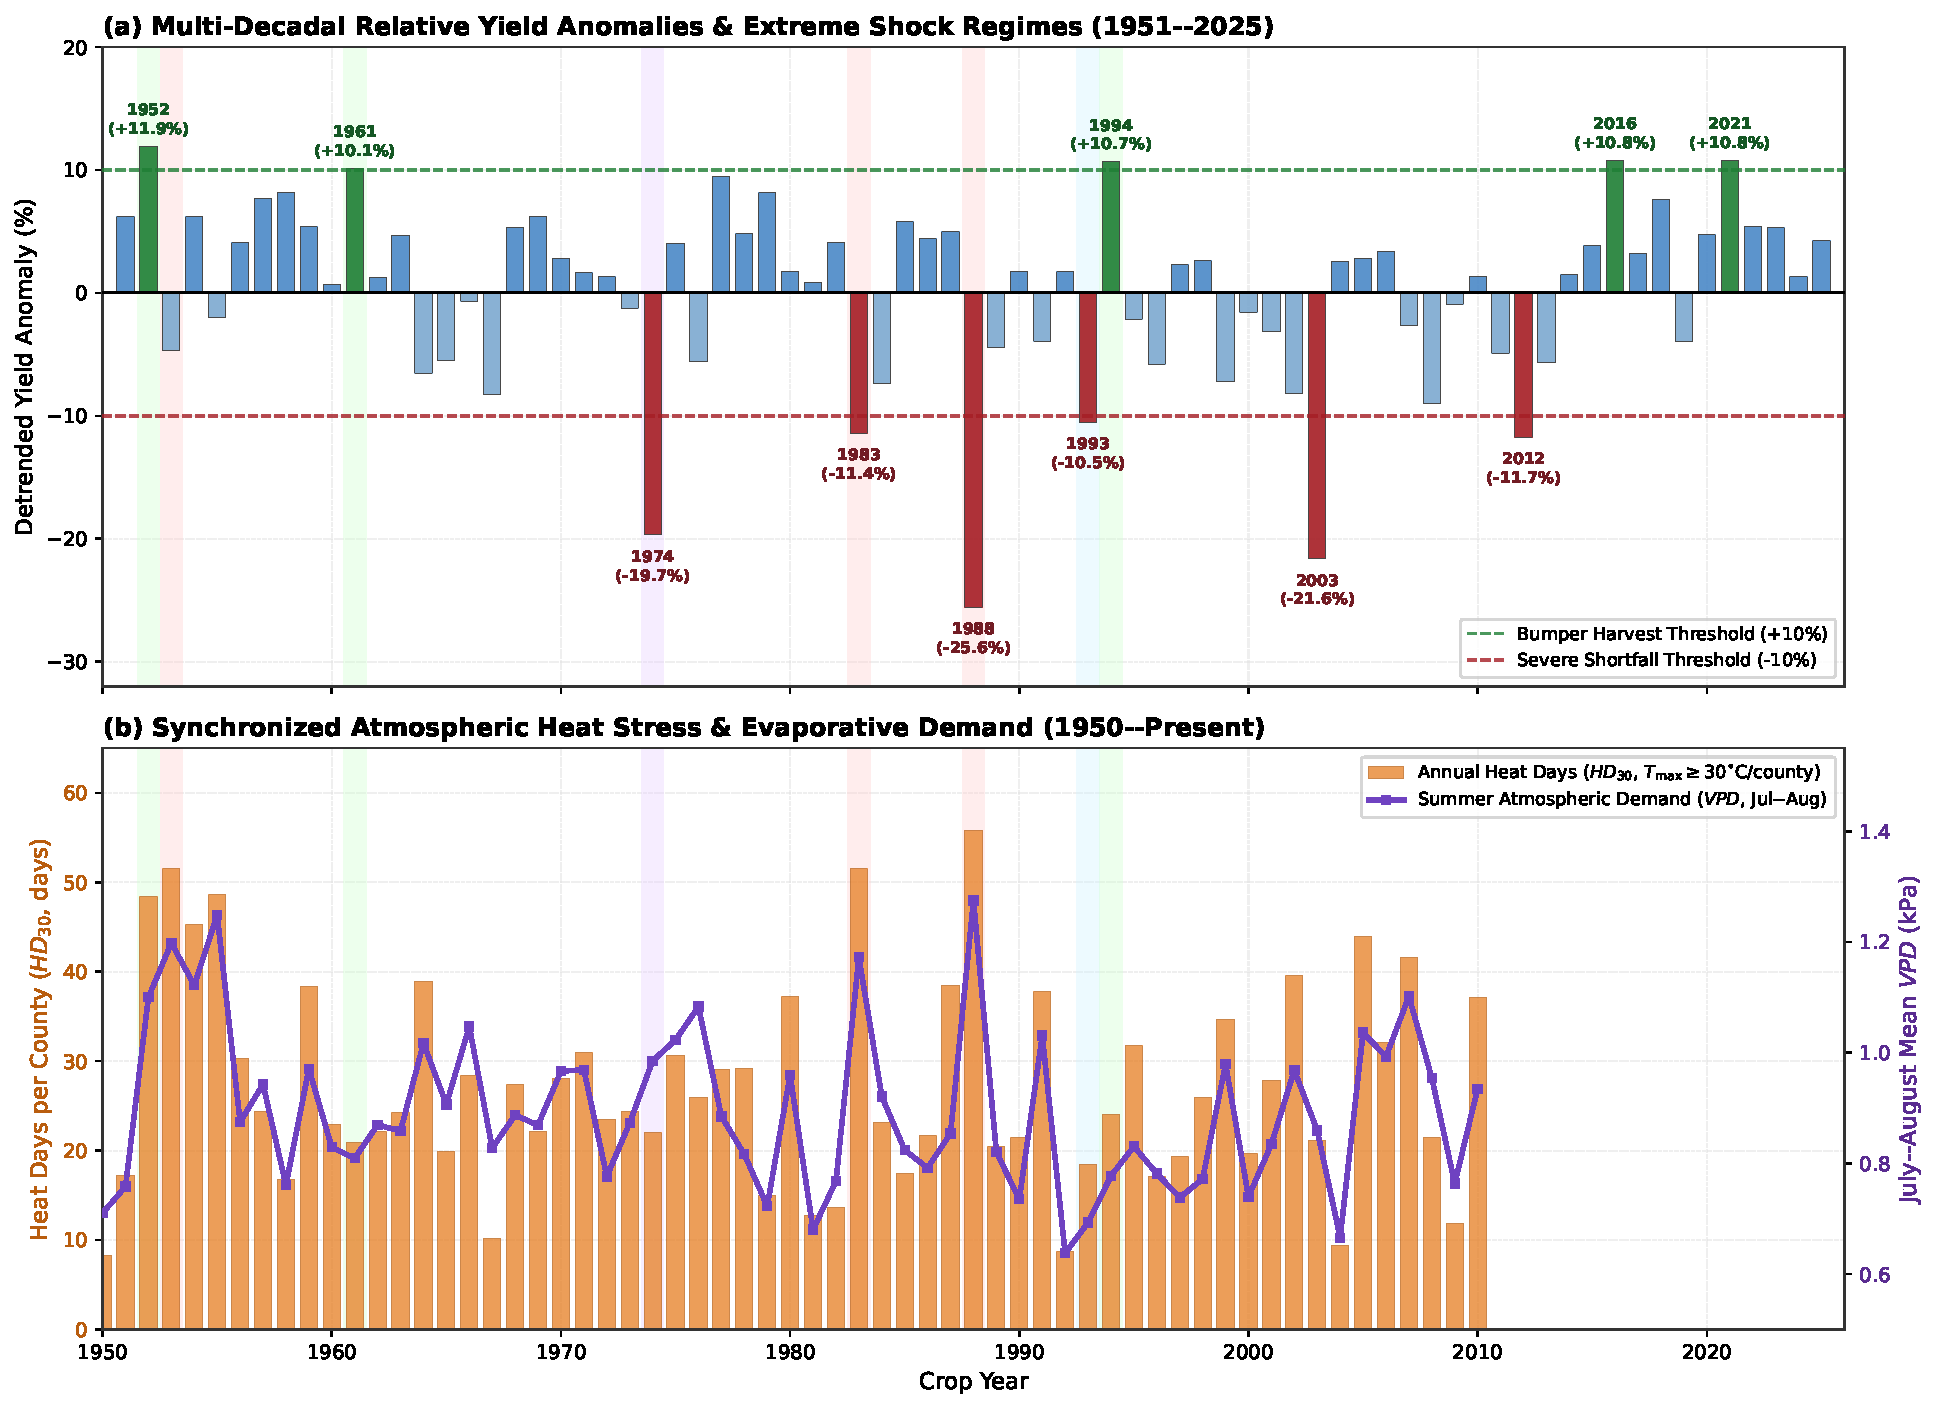
\includegraphics[width=0.96\textwidth]{figures/fig_weather_climatology}
    \caption{Multi-decadal agro-climatic stress evolution and county soybean yield shock nexus across 135 Midwestern study counties (1950--present). Panel (a) illustrates annual cross-sectional detrended yield anomalies relative to the secular linear trend, with prominent bumper harvests highlighted in emerald green ($\ge +10\%$) and catastrophic negative shortfalls in deep crimson ($\le -10\%$), bounded by explicit $\pm 10\%$ threshold guide lines. Panel (b) depicts annual extreme heat stress days ($HD_{30}$, days with $T_{\text{max}} \ge 30^\circ\text{C}$ per county, orange bars) and summer vapor pressure deficit ($VPD$, July--August mean, purple curve on secondary axis). Shaded vertical guide bands connect extreme anomaly years directly between panels, highlighting distinct thermal, hydrological, and biotic hazard mechanisms.}
    \label{fig:weather_climatology}
\end{figure}

The synchronized historical record resolves two foundational macro-climatic insights across the 75-year panel:

First, the most catastrophic regional harvest failures cluster tightly with historical apexes in compound atmospheric stress. Across multiple distinct historical decades—most notably the prolonged mid-century drought cycle (1953--1954), the acute mid-1980s events (1983, 1988), and the severe 2012 flash drought—annual heat-stress days surged past $50$ to $56\text{ days}$ per county, while summer vapor pressure deficit reached historic peaks of $1.2$ to $1.3\text{ kPa}$. In these high-stress regimes, intense thermal forcing and severe atmospheric evaporative demand act simultaneously, rapidly draining root-zone moisture reserves, terminating transpirational cooling, and aborting reproductive sinks \citep{Schlenker2009}. Conversely, across seven decades of technological progress, prominent bumper harvest clusters (such as 1952, 1961, 1979, 1994, 2016, and 2021) consistently coincide with suppressed heat accumulation ($HD_{30} < 20\text{ days}$) and benign summer evaporative demand ($VPD < 0.9\text{ kPa}$), preserving canopy hydration throughout reproductive development.

Second, the multi-decadal time series demonstrates that severe downside shocks do not originate exclusively from heatwaves and summer droughts. Significant regional shortfalls also emerge from distinct non-thermal and temporal hazard regimes:
\begin{itemize}
    \item \textit{Hydrological Inundation and Root Anoxia:} In pluvial disaster campaigns—most prominently 1993, but also observed in localized flood years such as 1958 and 2008—summer heat days ($HD_{30} \approx 8\text{ days}$) and $VPD$ ($0.71\text{ kPa}$) collapsed to multi-decadal minimums under persistent overcast storm tracks. Yield shortfalls ($-10.5\%$) were driven by continuous topsoil inundation, prolonged root-zone anoxia, impaired rhizobial nitrogen fixation, and rampant soil-borne fungal pathogens.
    \item \textit{Temporal Planting Delays and Cold Truncation:} In seasons characterized by compound temporal boundary hazards—such as 1974 ($-19.7\%$ shortfall) and 2019—torrential spring rainfall delayed field preparation and seeding by nearly a month. Although subsequent summer thermal conditions were moderate, the delayed reproductive calendar left immature canopies fully exposed to unseasonably early Arctic cold fronts, terminating dry-matter accumulation before physiological maturity.
    \item \textit{Compound Biotic-Abiotic Pressures:} Moderate meteorological stress can produce catastrophic yield collapses when interacting with biological vectors, as demonstrated by the 2003 shortfall ($-21.6\%$), where late-summer moisture deficits coincided with the first widespread North American epidemic of the invasive soybean aphid (\textit{Aphis glycines}).
\end{itemize}

\subsection{Intra-Seasonal Dynamics and Agro-Climatic Shock Archetypes}
\label{sec:data_intra_seasonal_extremes}

While multi-decadal time series establish long-term synchrony between atmospheric forcing and crop yields, understanding how meteorological anomalies propagate into realized county shortfalls requires tracing their intra-seasonal daily trajectories and normalized anomaly signatures. Across the 214 days of the primary growing cycle (April 1 to October 31), Figure~\ref{fig:intra_seasonal_extremes} details the daily physical progression of benchmark crop years across thermal accumulation ($HD_{30}$), evaporative demand ($VPD$), cumulative water balance ($P - ET_0$), and root-zone soil moisture ($SM_{\text{root}}$). In parallel, Figure~\ref{fig:weather_shocks_footprint} isolates their 15-day centered rolling anomalies relative to the historical climatological normal, providing a comparative footprint of environmental stress.

\begin{figure}[htbp]
    \centering
    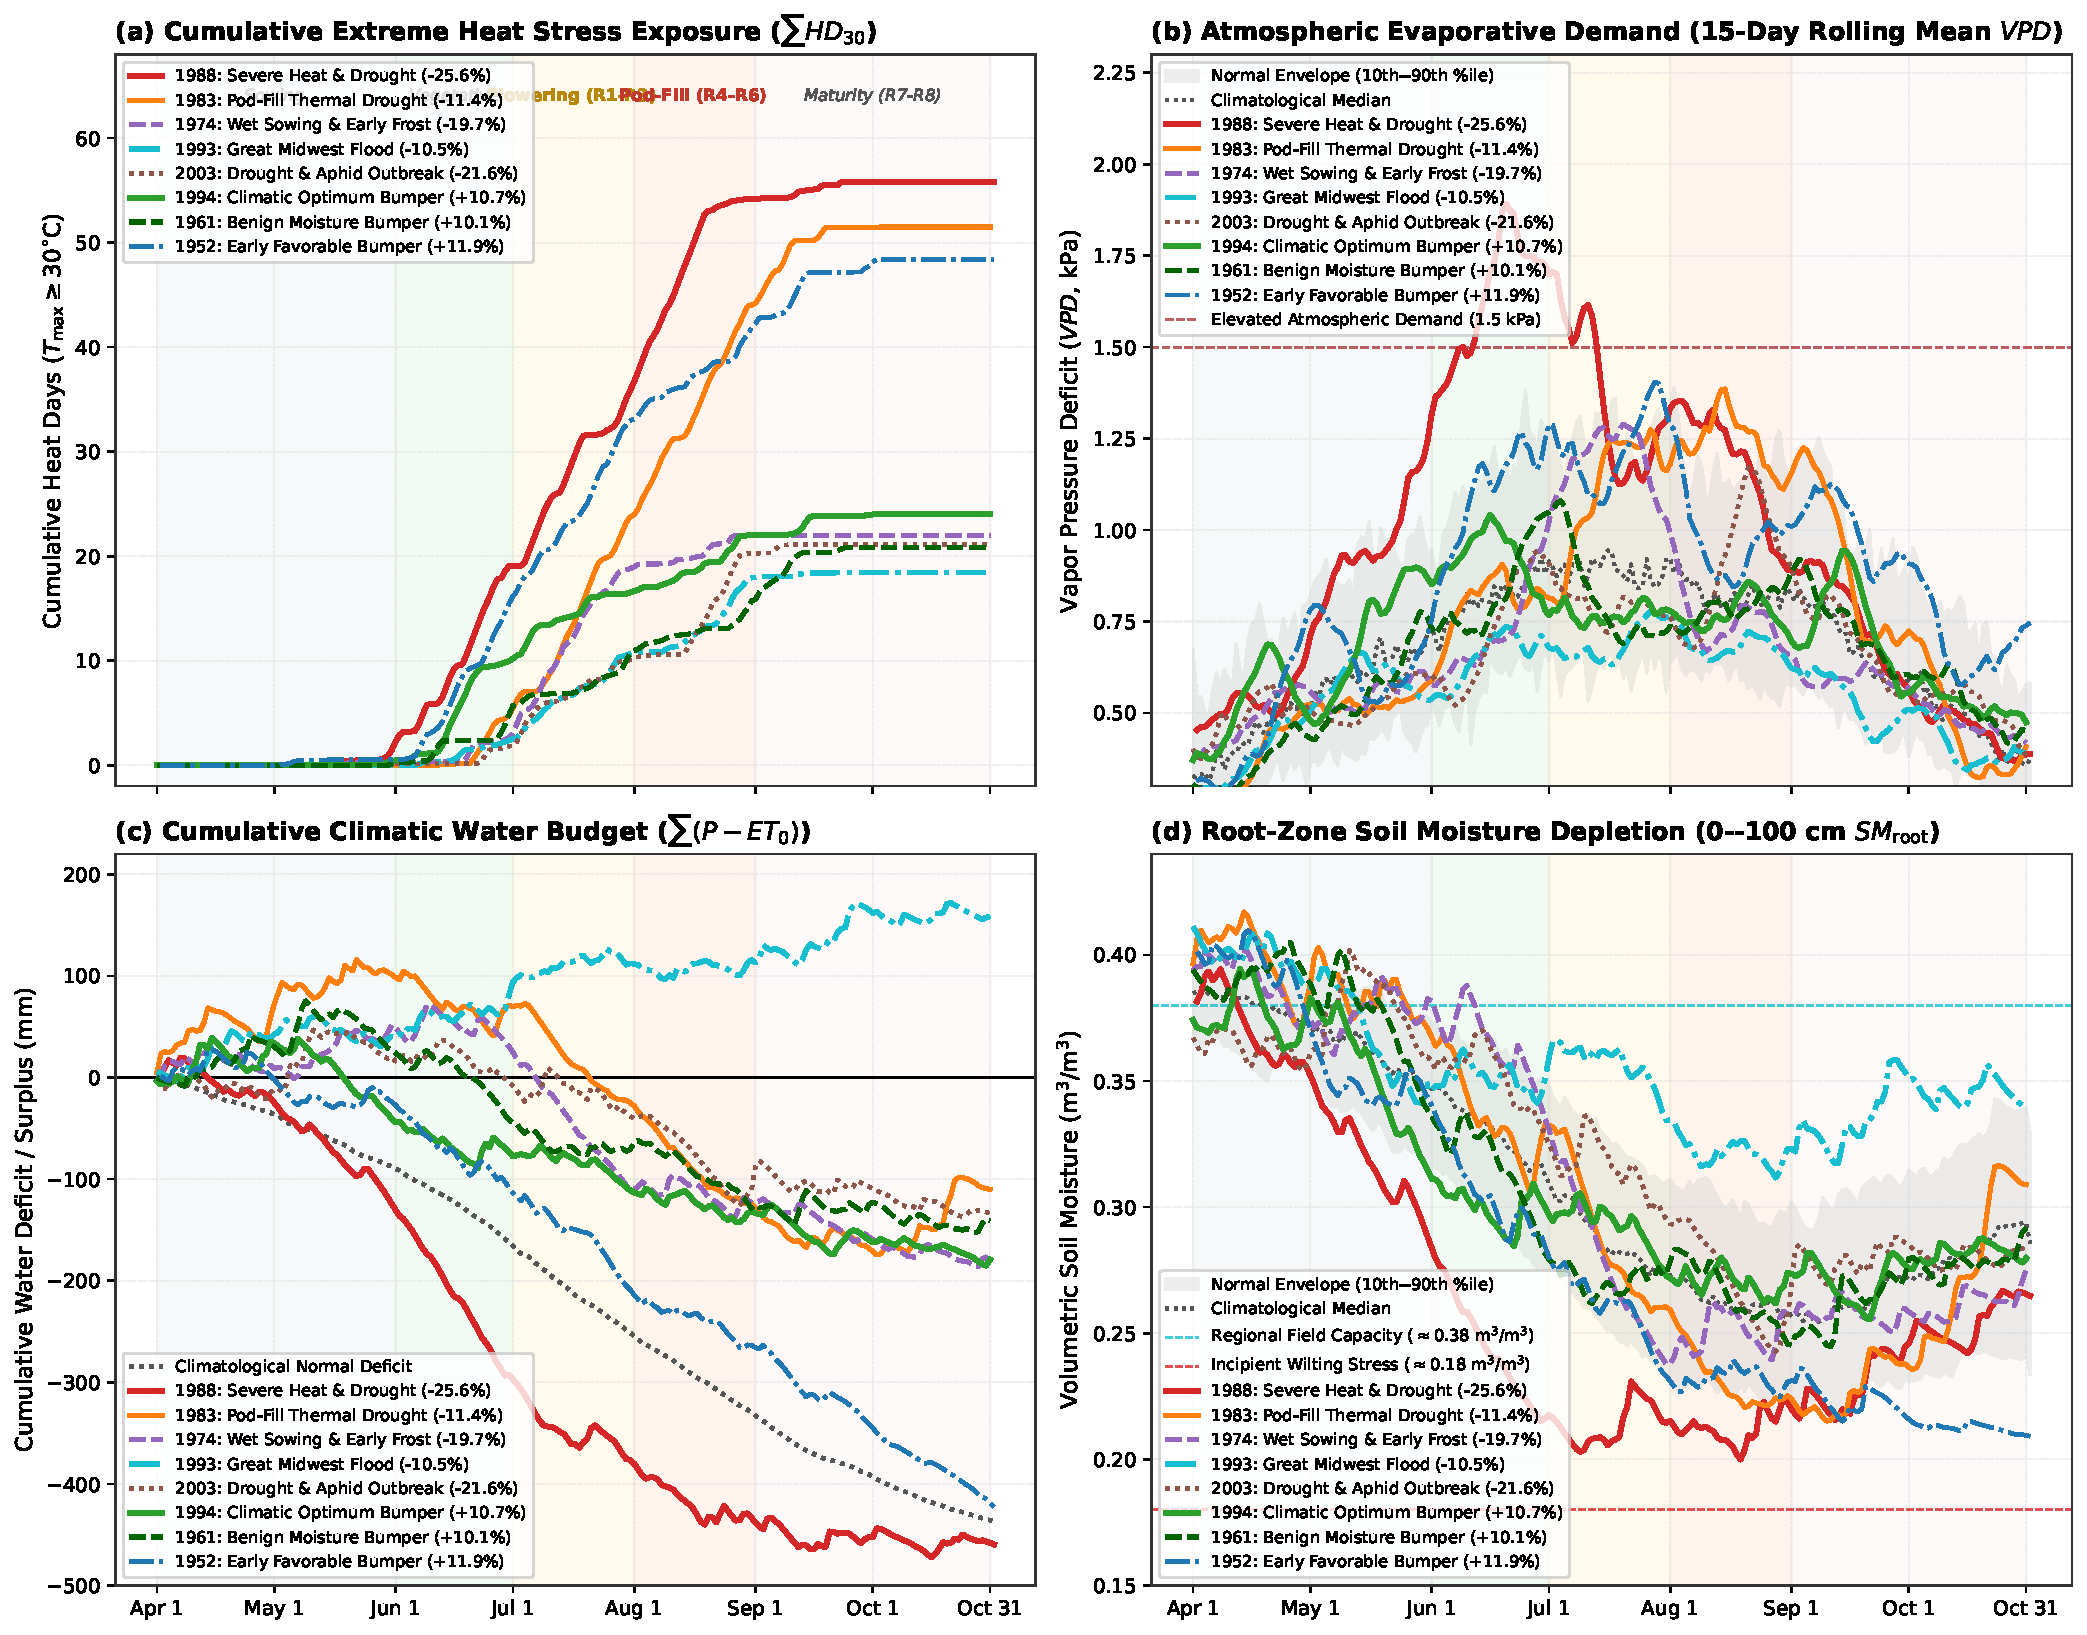
\includegraphics[width=0.96\textwidth]{figures/fig_intra_seasonal_extremes}
    \caption{Intra-seasonal phenological progression of historical extreme soybean yield years ($\pm 10\%$ threshold) across the Midwestern Corn Belt (April 1 to October 31). Panel (a) tracks cumulative extreme heat stress days ($\sum HD_{30}$, $T_{\text{max}} \ge 30^\circ\text{C}$). Panel (b) illustrates atmospheric evaporative demand via 15-day rolling mean $VPD$ against elevated demand ($1.5\text{ kPa}$) and the normal 10th--90th percentile envelope. Panel (c) traces the cumulative climatic water budget ($\sum (P - ET_0)$), contrasting catastrophic drought desiccation against flood waterlogging. Panel (d) displays depth-weighted root-zone soil moisture ($SM_{\text{root}}$, $0$--$100\text{ cm}$) against regional field capacity and incipient wilting stress. Trajectories distinguish individual negative shocks (1988, 1983, 1974, 1993, 2003) and positive bumper crops (1994, 1961, 1952).}
    \label{fig:intra_seasonal_extremes}
\end{figure}

\begin{figure}[htbp]
    \centering
    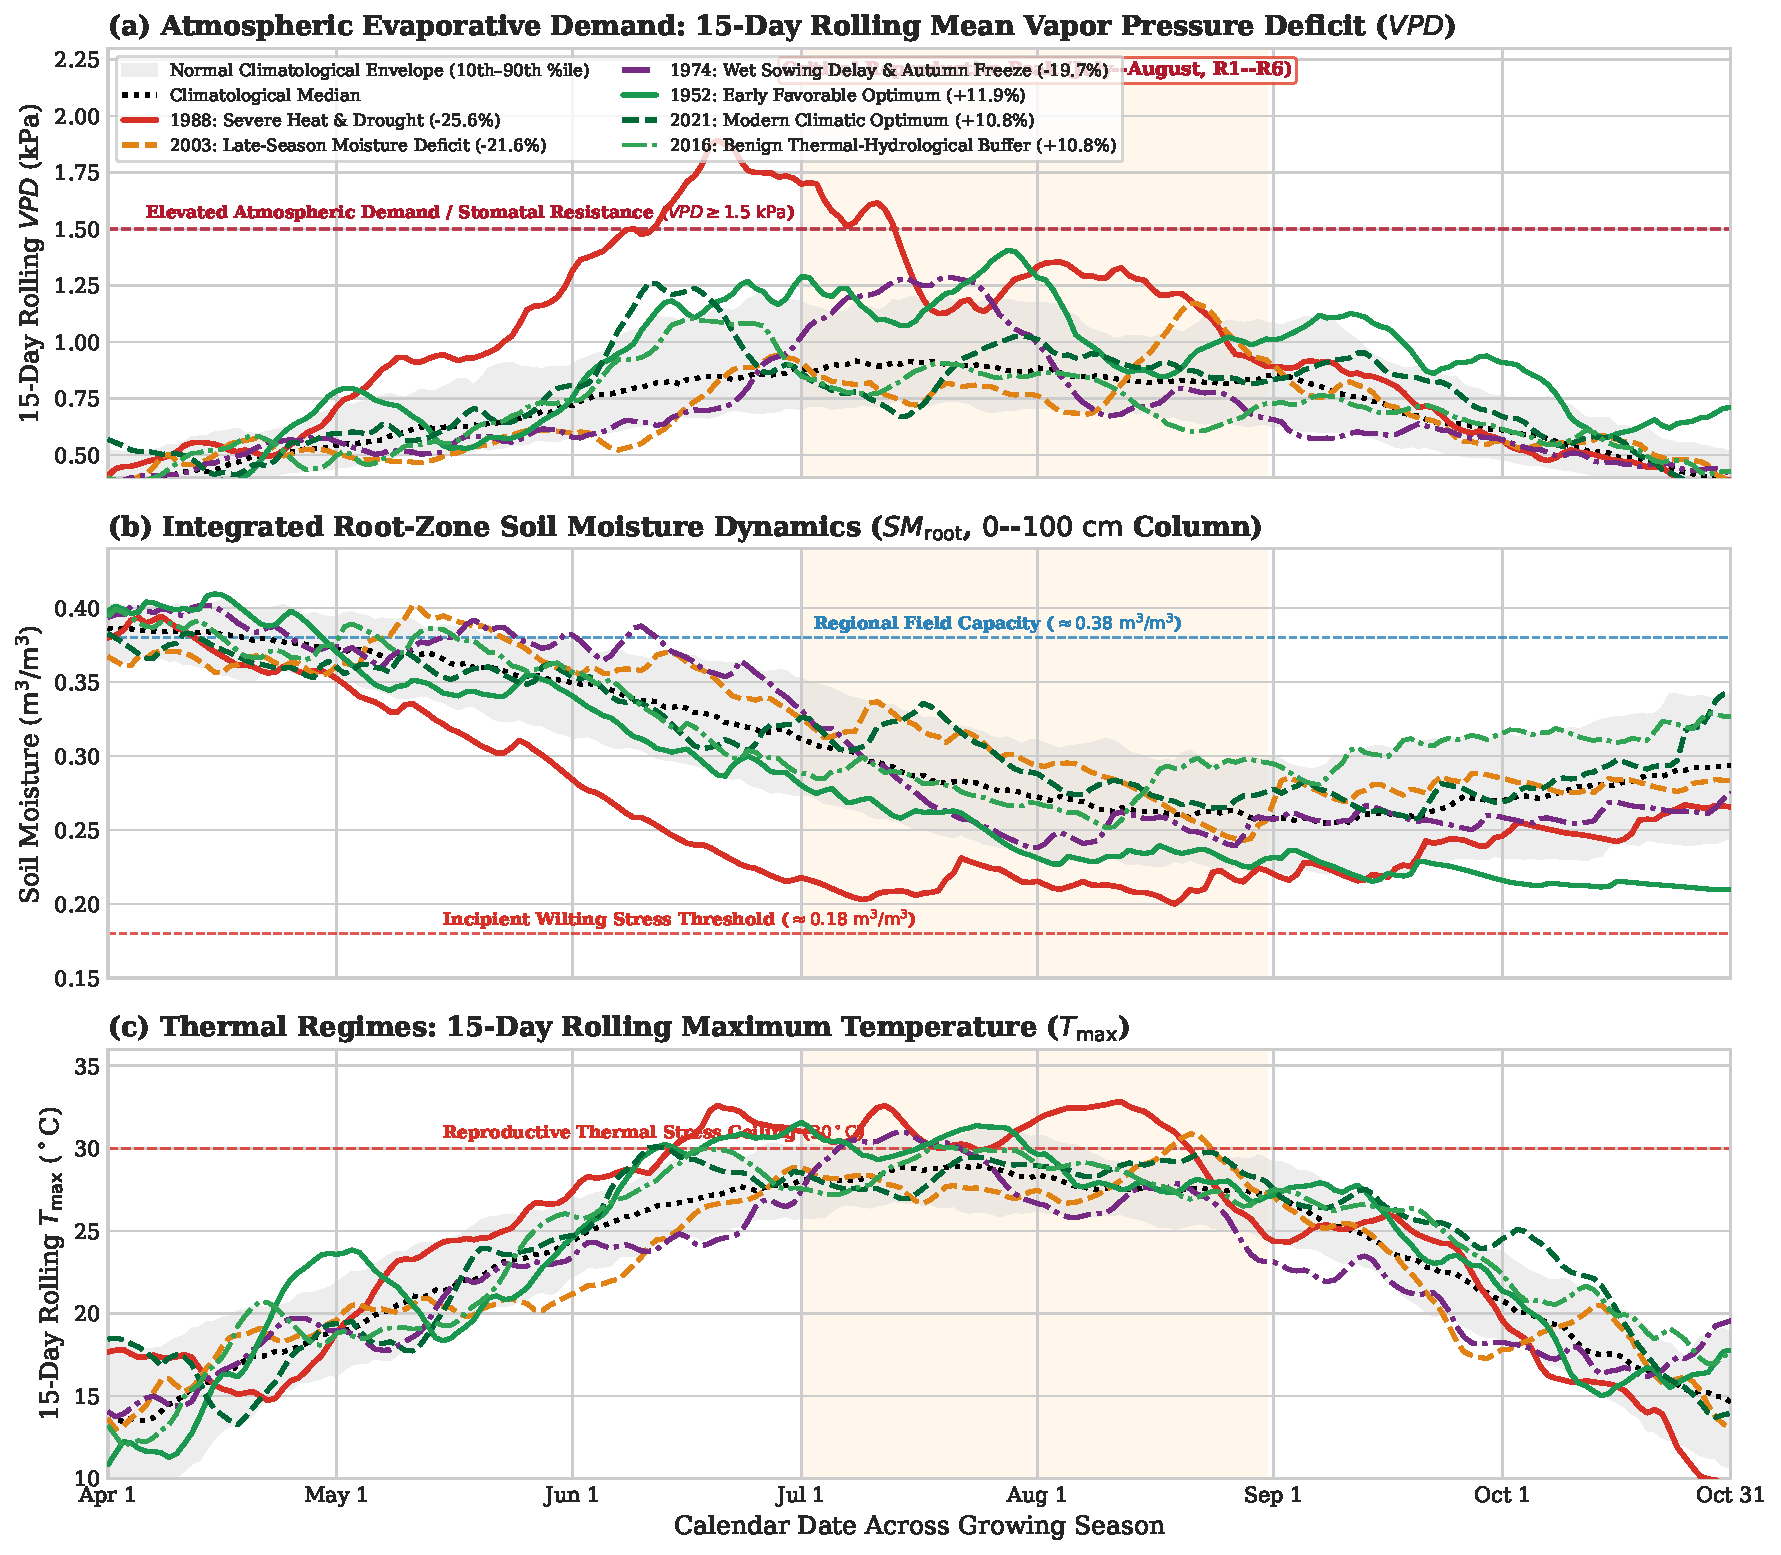
\includegraphics[width=0.96\textwidth]{figures/fig_weather_shocks_footprint}
    \caption{Comparative agro-climatic shock anomaly footprints across the soybean growing cycle (April--October) for representative historical archetypes: 1988 (severe summer heat and drought), 1983 (late-season pod-fill drought), 1974 (delayed wet sowing and early autumn freeze), 1993 (The Great Midwest Flood / soil waterlogging), and 1994 (climatic optimum / bumper harvest). Curves depict 15-day centered rolling anomalies relative to the historical panel climatology for precipitation ($P$), vapor pressure deficit ($VPD$), root-zone soil moisture ($SM_{\text{root}}$), and extreme heat days ($HD_{30}$).}
    \label{fig:weather_shocks_footprint}
\end{figure}

Synthesizing the daily trajectories and anomaly footprints reveals that historical extremes fall into four coherent agro-climatic cohorts:

\paragraph{Cohort I: Compound Thermal-Drought Stress.}
Drought-stressed campaigns across Midwestern history (including 1953, 1954, 1983, 1988, and 2012) are driven by persistent upper-tropospheric anticyclonic blocking ridges that displace frontal storm tracks northward. However, within this broad cohort, the daily trajectories resolve two critically distinct temporal stress profiles:
\begin{itemize}
    \item \textit{Chronic Full-Season Drought (e.g., 1988, 1953):} Meteorological deficits establish early in May and June, with rainfall anomalies running $-40$ to $-50\text{ mm/month}$ below normal throughout the summer (Figure~\ref{fig:weather_shocks_footprint}). Evaporative demand surges continuously ($VPD$ anomalies $> +0.8\text{ kPa}$), while heat-stress days accumulate steadily from mid-June to reach an unprecedented 56 days (Figure~\ref{fig:intra_seasonal_extremes}a). The cumulative climatic moisture deficit plunges below $-450\text{ mm}$, exhausting root-zone moisture reserves down to severe depletion levels ($<0.18\text{ m}^3/\text{m}^3$) well before seed filling, causing stunted vegetative frames and massive flower abortion.
    \item \textit{Reproductive Flash Drought and Pod-Fill Collapse (e.g., 1983, 2012):} In sharp contrast, vegetative development through May and June experiences near-normal rainfall and moderate temperatures, fostering expansive canopy development and high transpirational demand. In late July, however, an abrupt synoptic blocking ridge collapses precipitation to near zero and triggers an acute thermal surge ($HD_{30} > +5\text{ days/month}$, $VPD > +0.7\text{ kPa}$) directly coincident with pod fill (R4--R6, Figure~\ref{fig:weather_shocks_footprint}). The lush vegetative biomass rapidly drains remaining subsoil moisture, precipitating severe pod abortion, incomplete pod filling, and shriveled grain. These dynamics confirm that robust vegetative vigor offers zero buffer against acute late-season moisture deficits.
\end{itemize}

\paragraph{Cohort II: Pluvial Excess and Hydrological Saturation.}
Pluvial disaster seasons across the historical record (e.g., 1958, 1993, 2008, 2015) exhibit physical trajectories that represent the polar antithesis of drought. Cumulative heat days plateau at minimal levels ($\sum HD_{30} < 18\text{ days}$), while high relative humidity and cloud cover depress $VPD$ to $0.50$--$0.75\text{ kPa}$ (Figure~\ref{fig:intra_seasonal_extremes}a,b). Instead, persistent zonal storm tracks generate immense rainfall surpluses ($+60$ to $+100\text{ mm/month}$ above normal, Figure~\ref{fig:weather_shocks_footprint}), driving cumulative $P - ET_0$ past $+160\text{ mm}$. Root-zone soil moisture remains pinned at absolute saturation ($>0.40\text{ m}^3/\text{m}^3$). This sustained inundation suffocates root respiration, impairs symbiotic rhizobial nitrogen fixation, fosters extensive Phytophthora root rots, and leaves heavy machinery unable to enter saturated fields.

\paragraph{Cohort III: Temporal Boundary and Cold Truncation Hazards.}
Seasons governed by temporal boundary shocks (e.g., 1974, 2019) demonstrate that agricultural productivity can be severely impaired without anomalous midsummer heat or midsummer drought. In these campaigns, torrential spring precipitation saturates topsoils throughout April and May, delaying regional sowing operations by 3--4 weeks into June (Figure~\ref{fig:intra_seasonal_extremes}c). While midsummer temperatures and water balances remain moderate, this operational delay shifts the reproductive pod-fill calendar late into August and September. In late September, an unseasonably early Arctic cold front brings hard sub-freezing temperatures ($T_{\text{min}} < -2^\circ\text{C}$) across the northern and central Corn Belt (Figure~\ref{fig:weather_shocks_footprint}). The freeze abruptly kills the canopy before physiological maturity (R7), arresting carbohydrate translocation and permanently freezing immature green seeds in their pods.

\paragraph{Cohort IV: Agro-Climatic Optima and Bumper Harvest Regimes.}
Prominent bumper harvest cohorts across diverse technological eras (e.g., 1952, 1961, 1979, 1994, 2016, 2021) follow an ideal agro-climatic middle path. Daily temperatures remain remarkably mild, with daytime maxima consistently below $28^\circ\text{C}$ and cumulative heat-stress days plateauing below 20 days (Figure~\ref{fig:intra_seasonal_extremes}a). Atmospheric evaporative demand hovers smoothly within the transpirational optimum ($VPD \approx 0.75$--$1.0\text{ kPa}$), preventing midday stomatal closure while supporting vigorous carbon assimilation. Crucially, timely and well-distributed convective rainfall events replenish root-zone soil moisture at regular 7- to 10-day intervals without creating waterlogged conditions, maintaining $SM_{\text{root}}$ securely between $0.27$ and $0.34\text{ m}^3/\text{m}^3$ throughout the critical August seed-filling window (Figure~\ref{fig:intra_seasonal_extremes}d). Under these benign conditions, crops achieve the maximum photosynthetic yield permitted by the biological ceiling of C3 RuBisCO kinetics.

\subsection{Phenological Climate-Yield Sensitivity and Lead-Time Dynamics}
\label{sec:data_pheno_sensitivity}

To quantify the evolving empirical dependency between atmospheric anomalies and county soybean yields across the growing season, Figure~\ref{fig:climate_yield_sensitivity} presents bivariate Pearson correlation coefficients ($r$) computed between detrended yield anomalies ($\epsilon_{c,t}$) and monthly atmospheric anomalies across the 135 study counties.

\begin{figure}[htbp]
    \centering
    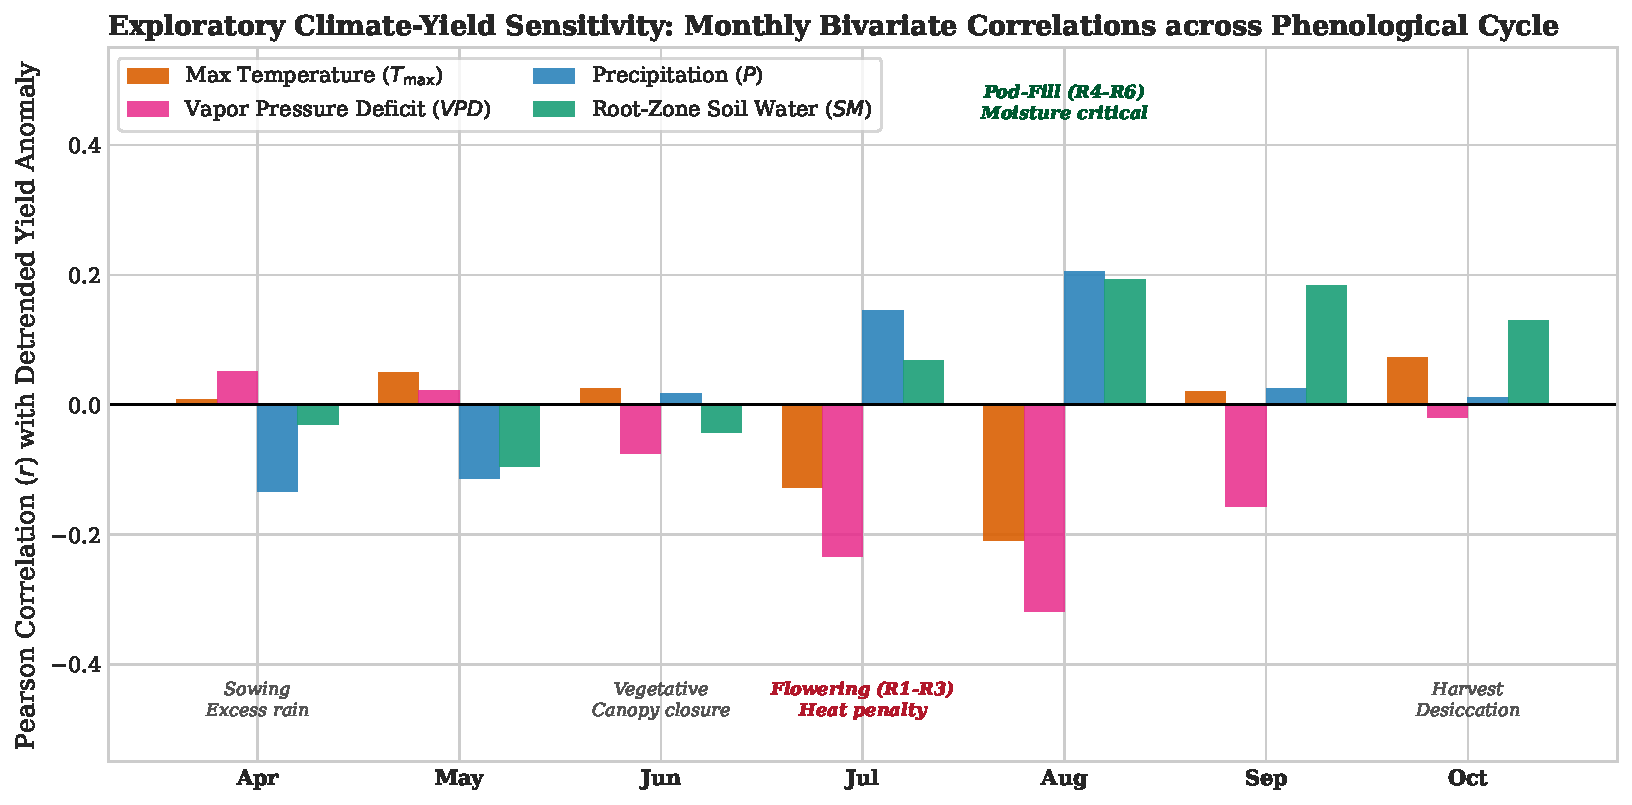
\includegraphics[width=0.96\textwidth]{figures/fig_climate_yield_sensitivity}
    \caption{Phenological sensitivity of county soybean yields to monthly atmospheric anomalies across the crop cycle (April--October). Bars depict cross-sectional Pearson correlation coefficients ($r$) between detrended yield anomalies ($\epsilon_{c,t}$) and monthly anomalies of maximum temperature ($T_{\text{max}}$), vapor pressure deficit ($VPD$), precipitation ($P$), and root-zone soil moisture ($SM_{\text{root}}$). Yield sensitivity is minimal during pre-sowing and emergence (April--May), escalates sharply during flowering (July), peaks during pod filling (August), and decays rapidly upon physiological maturity (September--October).}
    \label{fig:climate_yield_sensitivity}
\end{figure}

The empirical sensitivity profiles display four distinct phenological stages:
\begin{enumerate}
    \item \textbf{Pre-Sowing and Emergence Window (April--May):} Correlation coefficients between yield anomalies and weather variables are uniformly low ($|r| < 0.10$). Notably, precipitation and soil moisture exhibit slightly negative correlations with final yield ($r \approx -0.06$ to $-0.09$). This counter-intuitive negative relationship reflects the operational penalties of excessive spring moisture: wet fields delay field preparation and seeding, promote soil compaction, and foster early seedling diseases. Ambient temperature exerts negligible influence during this preparatory phase.
    \item \textbf{Vegetative Growth and Canopy Closure (June):} As crops establish root systems and leaf area, the sign of environmental sensitivities shifts toward positive moisture dependency. However, correlation magnitudes remain moderate ($r \approx +0.12$ for soil moisture; $r \approx -0.14$ for $VPD$), indicating that soybeans possess sufficient vegetative plasticity to recover from early-season weather aberrations if subsequent reproductive conditions are favorable.
    \item \textbf{Peak Reproductive Sensitivity (July--August):} Atmospheric sensitivity escalates dramatically during flowering (July, R1--R3) and reaches its maximum amplitude during pod development and seed filling (August, R4--R6). In August, the correlation between yield anomalies and root-zone soil moisture surges to $r = +0.43$, accompanied by precipitation at $r = +0.38$. Concurrently, atmospheric stress metrics exhibit severe negative correlations: $VPD$ reaches $r = -0.46$ and $T_{\text{max}}$ reaches $r = -0.41$. The co-occurrence of maximum evaporative demand ($VPD$) and reproductive seed swelling makes August weather the single most critical determinant of interannual yield variance.
    \item \textbf{Maturation and Senescence (September--October):} Following the completion of seed fill in late August, soybean leaves undergo rapid monocarpic senescence and yellowing (R7), followed by physiological maturity (R8) and field dry-down. Consequently, correlation coefficients plunge precipitously back toward zero ($|r| \le 0.05$ across all four variables). Atmospheric conditions in September and October affect grain moisture content and combine harvest efficiency, but exert zero biological impact on realized seed quantity.
\end{enumerate}

\paragraph{Methodological Implications for Progressive Lead-Time Forecasting.} The empirical sensitivity dynamics synthesized in Figure~\ref{fig:climate_yield_sensitivity} provide the direct scientific foundation for the progressive lead-time forecasting framework formalized in Chapter~4. 

At long presowing lead times ($H = 12, \dots, 6$, October through April), atmospheric forcings exhibit low direct correlation with final yield anomalies; predictive skill at these horizons must rely primarily on persistent antecedent root-zone soil moisture recharge and multi-month hydrological memory \citep{Vijverberg2023}. As the forecast horizon advances through vegetative development ($H = 5, 4$, May and June), incoming meteorological information gradually updates crop potential, but the system remains subject to high downstream epistemic uncertainty. 

The primary leap in physical predictability occurs at mid-season and late-summer horizons ($H = 3, 2$, July 31 and August 31), when predictive models ingest the realized atmospheric stress profile during the critical flowering and pod-fill windows. Finally, at horizon $H = 1$ (September 30), the biological crop yield is essentially fixed; remaining forecast uncertainty is dominated by localized combine harvest losses and late frost hazards rather than physiological yield formation. The mathematical formalization of these twelve discrete forecasting horizons, alongside the multi-granularity feature extraction and expanding-window validation protocols, is developed in Chapter~4.


% \include{chapters/04_methodology}
% \include{chapters/05_empirical_results}
% \include{chapters/06_discussion}
% \include{chapters/07_conclusions}

% ------------------------------------------------------------------------------
% Bibliography
% ------------------------------------------------------------------------------
\clearpage
\bibliographystyle{apalike}
\bibliography{references}

\end{document}
